\documentclass[twoside]{book}

% Packages required by doxygen
\usepackage{fixltx2e}
\usepackage{calc}
\usepackage{doxygen}
\usepackage[export]{adjustbox} % also loads graphicx
\usepackage{graphicx}
\usepackage[utf8]{inputenc}
\usepackage{makeidx}
\usepackage{multicol}
\usepackage{multirow}
\PassOptionsToPackage{warn}{textcomp}
\usepackage{textcomp}
\usepackage[nointegrals]{wasysym}
\usepackage[table]{xcolor}

% Font selection
\usepackage[T1]{fontenc}
\usepackage[scaled=.90]{helvet}
\usepackage{courier}
\usepackage{amssymb}
\usepackage{sectsty}
\renewcommand{\familydefault}{\sfdefault}
\allsectionsfont{%
  \fontseries{bc}\selectfont%
  \color{darkgray}%
}
\renewcommand{\DoxyLabelFont}{%
  \fontseries{bc}\selectfont%
  \color{darkgray}%
}
\newcommand{\+}{\discretionary{\mbox{\scriptsize$\hookleftarrow$}}{}{}}

% Page & text layout
\usepackage{geometry}
\geometry{%
  a4paper,%
  top=2.5cm,%
  bottom=2.5cm,%
  left=2.5cm,%
  right=2.5cm%
}
\tolerance=750
\hfuzz=15pt
\hbadness=750
\setlength{\emergencystretch}{15pt}
\setlength{\parindent}{0cm}
\setlength{\parskip}{3ex plus 2ex minus 2ex}
\makeatletter
\renewcommand{\paragraph}{%
  \@startsection{paragraph}{4}{0ex}{-1.0ex}{1.0ex}{%
    \normalfont\normalsize\bfseries\SS@parafont%
  }%
}
\renewcommand{\subparagraph}{%
  \@startsection{subparagraph}{5}{0ex}{-1.0ex}{1.0ex}{%
    \normalfont\normalsize\bfseries\SS@subparafont%
  }%
}
\makeatother

% Headers & footers
\usepackage{fancyhdr}
\pagestyle{fancyplain}
\fancyhead[LE]{\fancyplain{}{\bfseries\thepage}}
\fancyhead[CE]{\fancyplain{}{}}
\fancyhead[RE]{\fancyplain{}{\bfseries\leftmark}}
\fancyhead[LO]{\fancyplain{}{\bfseries\rightmark}}
\fancyhead[CO]{\fancyplain{}{}}
\fancyhead[RO]{\fancyplain{}{\bfseries\thepage}}
\fancyfoot[LE]{\fancyplain{}{}}
\fancyfoot[CE]{\fancyplain{}{}}
\fancyfoot[RE]{\fancyplain{}{\bfseries\scriptsize Generated by Doxygen }}
\fancyfoot[LO]{\fancyplain{}{\bfseries\scriptsize Generated by Doxygen }}
\fancyfoot[CO]{\fancyplain{}{}}
\fancyfoot[RO]{\fancyplain{}{}}
\renewcommand{\footrulewidth}{0.4pt}
\renewcommand{\chaptermark}[1]{%
  \markboth{#1}{}%
}
\renewcommand{\sectionmark}[1]{%
  \markright{\thesection\ #1}%
}

% Indices & bibliography
\usepackage{natbib}
\usepackage[titles]{tocloft}
\setcounter{tocdepth}{3}
\setcounter{secnumdepth}{5}
\makeindex

% Hyperlinks (required, but should be loaded last)
\usepackage{ifpdf}
\ifpdf
  \usepackage[pdftex,pagebackref=true]{hyperref}
\else
  \usepackage[ps2pdf,pagebackref=true]{hyperref}
\fi
\hypersetup{%
  colorlinks=true,%
  linkcolor=blue,%
  citecolor=blue,%
  unicode%
}

% Custom commands
\newcommand{\clearemptydoublepage}{%
  \newpage{\pagestyle{empty}\cleardoublepage}%
}

\usepackage{caption}
\captionsetup{labelsep=space,justification=centering,font={bf},singlelinecheck=off,skip=4pt,position=top}

%===== C O N T E N T S =====

\begin{document}

% Titlepage & ToC
\hypersetup{pageanchor=false,
             bookmarksnumbered=true,
             pdfencoding=unicode
            }
\pagenumbering{alph}
\begin{titlepage}
\vspace*{7cm}
\begin{center}%
{\Large Spiffs\+Particle\+RK }\\
\vspace*{1cm}
{\large Generated by Doxygen 1.8.14}\\
\end{center}
\end{titlepage}
\clearemptydoublepage
\pagenumbering{roman}
\tableofcontents
\clearemptydoublepage
\pagenumbering{arabic}
\hypersetup{pageanchor=true}

%--- Begin generated contents ---
\chapter{Spiffs\+Particle\+RK}
\label{index}\hypertarget{index}{}{\itshape Port of the S\+P\+I\+F\+FS library for the Particle platform}

\subsection*{Introduction}

The \href{https://github.com/pellepl/spiffs}{\tt excellent S\+P\+I\+F\+FS library} provides a simple file system on a N\+OR flash chip. This is a port of the library for the Particle platform, with a few convenience helpers to make using it easier from C++ and using standard Particle/\+Arduino/\+Wiring A\+P\+Is.

Both the original S\+P\+I\+F\+FS library and this port and M\+IT licensed, so you can use them in open-\/source or in closed-\/source commercial products without a fee or license.

\subsection*{Flash Support}

This library supports S\+P\+I-\/connected N\+OR flash chips. These are typically tiny 8-\/\+S\+O\+IC surface mount chips, intended to be included on your own circuit board. There are also breadboard adapters that are available, shown in the examples below.

The chips are really inexpensive, less than US\$0.\+60 in single quantities for a 1 Mbyte flash. They\textquotesingle{}re available in sizes up to 16 Mbyte.

S\+PI flash is less expensive than SD cards, and do not need an adapter or card slot. Of course they\textquotesingle{}re not removable, either.

The underlying \href{https://github.com/rickkas7/SpiFlashRK}{\tt Spi\+Flash\+RK library} library supports S\+PI N\+OR flash from


\begin{DoxyItemize}
\item I\+S\+SI, such as a \href{http://www.digikey.com/product-detail/en/issi-integrated-silicon-solution-inc/IS25LQ080B-JNLE/706-1331-ND/5189766}{\tt I\+S25\+L\+Q080B}.
\item Winbond, such as a \href{https://www.digikey.com/product-detail/en/winbond-electronics/W25Q32JVSSIQ/W25Q32JVSSIQ-ND/5803981}{\tt W25\+Q32}.
\item Macronix, such as the \href{https://www.digikey.com/product-detail/en/macronix/MX25L8006EM1I-12G/1092-1117-ND/2744800}{\tt M\+X25\+L8006\+E\+M1\+I-\/12G}
\item The external 1 Mbyte flash on the P1 module
\item Probably others
\end{DoxyItemize}

It does not support I2C flash, SD cards, or non-\/flash chips like F\+R\+AM.

\subsection*{Instantiating an Spi\+Flash object}

You typically instantiate an object to interface to the flash chip as a global variable\+:


\begin{DoxyCode}
SpiFlashISSI spiFlash(SPI, A2);
\end{DoxyCode}


I\+S\+SI flash connected to the primary S\+PI with A2 as the CS (chip select or SS).


\begin{DoxyCode}
SpiFlashWinbond spiFlash(SPI, A2);
\end{DoxyCode}


Winbond flash connected to the primary S\+PI with A2 as the CS (chip select or SS).


\begin{DoxyCode}
SpiFlashWinbond spiFlash(SPI1, D5);
\end{DoxyCode}


Winbond flash connected to the secondary S\+PI, S\+P\+I1, with D5 as the CS (chip select or SS).


\begin{DoxyCode}
SpiFlashMacronix spiFlash(SPI1, D5);
\end{DoxyCode}


Macronix flash connected to the secondary S\+PI, S\+P\+I1, with D5 as the CS (chip select or SS). This is the recommended for use on the E-\/\+Series module. Note that this is the 0.\+154", 3.\+90mm width 8-\/\+S\+O\+IC package.


\begin{DoxyCode}
SpiFlashP1 spiFlash;
\end{DoxyCode}


The external flash on the P1 module. This extra flash chip is entirely available for your user; it is not used by the system firmware. You can only use this on the P1; it relies on system functions that are not available on other devices.

\subsection*{Connecting the hardware}

The real intention is to reflow the 8-\/\+S\+O\+IC module directly to your custom circuit board. However, for prototyping, here are some examples\+:

For the primary S\+PI (S\+PI)\+:

\tabulinesep=1mm
\begin{longtabu} spread 0pt [c]{*{4}{|X[-1]}|}
\hline
\rowcolor{\tableheadbgcolor}\textbf{ Name  }&\textbf{ Flash Alt Name  }&\textbf{ Particle Pin  }&\textbf{ Example Color   }\\\cline{1-4}
\endfirsthead
\hline
\endfoot
\hline
\rowcolor{\tableheadbgcolor}\textbf{ Name  }&\textbf{ Flash Alt Name  }&\textbf{ Particle Pin  }&\textbf{ Example Color   }\\\cline{1-4}
\endhead
SS  &CS  &A2  &White   \\\cline{1-4}
S\+CK  &C\+LK  &A3  &Orange   \\\cline{1-4}
M\+I\+SO  &DO  &A4  &Blue   \\\cline{1-4}
M\+O\+SI  &D1  &A5  &Green   \\\cline{1-4}
\end{longtabu}


For the secondary S\+PI (S\+P\+I1)\+:

\tabulinesep=1mm
\begin{longtabu} spread 0pt [c]{*{4}{|X[-1]}|}
\hline
\rowcolor{\tableheadbgcolor}\textbf{ Name  }&\textbf{ Flash Alt Name  }&\textbf{ Particle Pin  }&\textbf{ Example Color   }\\\cline{1-4}
\endfirsthead
\hline
\endfoot
\hline
\rowcolor{\tableheadbgcolor}\textbf{ Name  }&\textbf{ Flash Alt Name  }&\textbf{ Particle Pin  }&\textbf{ Example Color   }\\\cline{1-4}
\endhead
SS  &CS  &D5  &White   \\\cline{1-4}
S\+CK  &C\+LK  &D4  &Orange   \\\cline{1-4}
M\+I\+SO  &DO  &D3  &Blue   \\\cline{1-4}
M\+O\+SI  &D1  &D2  &Green   \\\cline{1-4}
\end{longtabu}


Note that the S\+S/\+CS line can be any available G\+P\+IO pin, not just the one specified in the table above.


\begin{DoxyItemize}
\item Electron using Primary S\+PI
\end{DoxyItemize}


\begin{DoxyItemize}
\item Photon using Secondary S\+PI (S\+P\+I1)
\end{DoxyItemize}


\begin{DoxyItemize}
\item Photon using Primary S\+PI and a poorly hand-\/soldered 8-\/\+S\+O\+IC adapter
\end{DoxyItemize}


\begin{DoxyItemize}
\item E-\/series evaluation kit with a \href{https://www.digikey.com/product-detail/en/macronix/MX25L8006EM1I-12G/1092-1117-ND/2744800}{\tt Macronix M\+X25\+L8006\+E\+M1\+I-\/12G} soldered to the E-\/series module (outlined in pink).
\end{DoxyItemize}


\begin{DoxyItemize}
\item P1 module (extra flash is under the can)
\end{DoxyItemize}

 \subsection*{Setting up the \mbox{\hyperlink{class_spiffs_particle}{Spiffs\+Particle}} object}

\subsection*{Using the S\+P\+I\+F\+FS A\+PI}

\subsubsection*{Background}

A few things about S\+P\+I\+F\+FS\+:


\begin{DoxyItemize}
\item It\textquotesingle{}s relatively small, way smaller than S\+D\+F\+AT at least.
\item It has the bare minimum of things you need to store files.
\item You can allocate all or part of the flash chip to S\+P\+I\+F\+FS.
\end{DoxyItemize}

In particular, there are two important limitations\+:


\begin{DoxyItemize}
\item It does not support subdirectories; all files are in a single directory.
\item Filenames are limited to 31 characters.
\item It does not have file timestamps (modification or creation times).
\end{DoxyItemize}

Within the scope of how you use S\+P\+I\+F\+FS these shouldn\textquotesingle{}t be unreasonable limitations, though you should be aware.

Like most file systems, there are a few things you must do\+:


\begin{DoxyItemize}
\item You must mount the file system, typically at startup.
\item If your flash is blank, you\textquotesingle{}ll need to format the file system.
\item You can iterate the top level directory to find the file names in it.
\item In order to use data in a file, you must open it and get a file handle, read or write, then close it.
\item There are a finite number of files that can be open, but you can set the maximum. The default is 4.
\item If you think the file system is corrupted, you can check and repair it.
\end{DoxyItemize}

Once you get it working, there is some fine-\/tuning you can do\+:


\begin{DoxyItemize}
\item The cache size is programmable, which speeds up operations at the cost of additional R\+AM. The default is 2 logical blocks.
\item The logical block size is programmable. Using larger blocks can make using large files more efficient in flash storage, at the cost of more R\+AM and making small files less efficient in flash storage. The default is 4K, and can\textquotesingle{}t be made smaller but can be made larger.
\end{DoxyItemize}

\subsection*{Using the Arduino/\+Wiring File A\+PI}

\subsection*{Resource usage}
\chapter{Hierarchical Index}
\section{Class Hierarchy}
This inheritance list is sorted roughly, but not completely, alphabetically\+:\begin{DoxyCompactList}
\item \contentsline{section}{Print}{\pageref{class_print}}{}
\begin{DoxyCompactList}
\item \contentsline{section}{Stream}{\pageref{class_stream}}{}
\begin{DoxyCompactList}
\item \contentsline{section}{Spiffs\+Particle\+File}{\pageref{class_spiffs_particle_file}}{}
\end{DoxyCompactList}
\end{DoxyCompactList}
\item \contentsline{section}{spiffs\+\_\+config}{\pageref{structspiffs__config}}{}
\item \contentsline{section}{spiffs\+\_\+\+D\+IR}{\pageref{structspiffs___d_i_r}}{}
\item \contentsline{section}{spiffs\+\_\+dirent}{\pageref{structspiffs__dirent}}{}
\item \contentsline{section}{spiffs\+\_\+fd}{\pageref{structspiffs__fd}}{}
\item \contentsline{section}{spiffs\+\_\+free\+\_\+obj\+\_\+id\+\_\+state}{\pageref{structspiffs__free__obj__id__state}}{}
\item \contentsline{section}{spiffs\+\_\+gc}{\pageref{structspiffs__gc}}{}
\item \contentsline{section}{spiffs\+\_\+ix\+\_\+map}{\pageref{structspiffs__ix__map}}{}
\item \contentsline{section}{spiffs\+\_\+ix\+\_\+map\+\_\+populate\+\_\+state}{\pageref{structspiffs__ix__map__populate__state}}{}
\item \contentsline{section}{S\+P\+I\+F\+F\+S\+\_\+\+P\+A\+C\+K\+ED}{\pageref{struct_s_p_i_f_f_s___p_a_c_k_e_d}}{}
\item \contentsline{section}{spiffs\+\_\+stat}{\pageref{structspiffs__stat}}{}
\item \contentsline{section}{spiffs\+\_\+t}{\pageref{structspiffs__t}}{}
\item \contentsline{section}{Spiffs\+Particle}{\pageref{class_spiffs_particle}}{}
\end{DoxyCompactList}

\chapter{Data Structure Index}
\section{Data Structures}
Here are the data structures with brief descriptions\+:\begin{DoxyCompactList}
\item\contentsline{section}{\mbox{\hyperlink{class_print}{Print}} \\*Class for printing to a stream or file }{\pageref{class_print}}{}
\item\contentsline{section}{\mbox{\hyperlink{structspiffs__config}{spiffs\+\_\+config}} }{\pageref{structspiffs__config}}{}
\item\contentsline{section}{\mbox{\hyperlink{structspiffs___d_i_r}{spiffs\+\_\+\+D\+IR}} }{\pageref{structspiffs___d_i_r}}{}
\item\contentsline{section}{\mbox{\hyperlink{structspiffs__dirent}{spiffs\+\_\+dirent}} }{\pageref{structspiffs__dirent}}{}
\item\contentsline{section}{\mbox{\hyperlink{structspiffs__fd}{spiffs\+\_\+fd}} }{\pageref{structspiffs__fd}}{}
\item\contentsline{section}{\mbox{\hyperlink{structspiffs__free__obj__id__state}{spiffs\+\_\+free\+\_\+obj\+\_\+id\+\_\+state}} }{\pageref{structspiffs__free__obj__id__state}}{}
\item\contentsline{section}{\mbox{\hyperlink{structspiffs__gc}{spiffs\+\_\+gc}} }{\pageref{structspiffs__gc}}{}
\item\contentsline{section}{\mbox{\hyperlink{structspiffs__ix__map}{spiffs\+\_\+ix\+\_\+map}} }{\pageref{structspiffs__ix__map}}{}
\item\contentsline{section}{\mbox{\hyperlink{structspiffs__ix__map__populate__state}{spiffs\+\_\+ix\+\_\+map\+\_\+populate\+\_\+state}} }{\pageref{structspiffs__ix__map__populate__state}}{}
\item\contentsline{section}{\mbox{\hyperlink{struct_s_p_i_f_f_s___p_a_c_k_e_d}{S\+P\+I\+F\+F\+S\+\_\+\+P\+A\+C\+K\+ED}} }{\pageref{struct_s_p_i_f_f_s___p_a_c_k_e_d}}{}
\item\contentsline{section}{\mbox{\hyperlink{structspiffs__stat}{spiffs\+\_\+stat}} }{\pageref{structspiffs__stat}}{}
\item\contentsline{section}{\mbox{\hyperlink{structspiffs__t}{spiffs\+\_\+t}} }{\pageref{structspiffs__t}}{}
\item\contentsline{section}{\mbox{\hyperlink{class_spiffs_particle}{Spiffs\+Particle}} \\*C++ wrapper for the S\+P\+I\+F\+FS library for the Particle platform }{\pageref{class_spiffs_particle}}{}
\item\contentsline{section}{\mbox{\hyperlink{class_spiffs_particle_file}{Spiffs\+Particle\+File}} \\*Extension of Arduino/\+Wiring Stream/\+Print manipulating a single S\+P\+I\+F\+FS file }{\pageref{class_spiffs_particle_file}}{}
\item\contentsline{section}{\mbox{\hyperlink{class_stream}{Stream}} \\*Arduino/\+Wiring \mbox{\hyperlink{class_stream}{Stream}} Class }{\pageref{class_stream}}{}
\end{DoxyCompactList}

\chapter{File Index}
\section{File List}
Here is a list of all documented files with brief descriptions\+:\begin{DoxyCompactList}
\item\contentsline{section}{docs/src/\mbox{\hyperlink{spark__wiring__print_8h}{spark\+\_\+wiring\+\_\+print.\+h}} \\*Header for spark\+\_\+wiring\+\_\+print.\+c module }{\pageref{spark__wiring__print_8h}}{}
\item\contentsline{section}{docs/src/\mbox{\hyperlink{spark__wiring__stream_8h}{spark\+\_\+wiring\+\_\+stream.\+h}} \\*Header for spark\+\_\+wiring\+\_\+stream.\+c module }{\pageref{spark__wiring__stream_8h}}{}
\item\contentsline{section}{src/{\bfseries spiffs.\+h} }{\pageref{spiffs_8h}}{}
\item\contentsline{section}{src/{\bfseries spiffs\+\_\+config.\+h} }{\pageref{spiffs__config_8h}}{}
\item\contentsline{section}{src/{\bfseries spiffs\+\_\+nucleus.\+h} }{\pageref{spiffs__nucleus_8h}}{}
\item\contentsline{section}{src/{\bfseries Spiffs\+Particle\+R\+K.\+h} }{\pageref{_spiffs_particle_r_k_8h}}{}
\item\contentsline{section}{src/{\bfseries Test\+Suite\+Impl.\+h} }{\pageref{_test_suite_impl_8h}}{}
\end{DoxyCompactList}

\chapter{Data Structure Documentation}
\hypertarget{class_print}{}\section{Print Class Reference}
\label{class_print}\index{Print@{Print}}


Class for printing to a stream or file.  




{\ttfamily \#include $<$spark\+\_\+wiring\+\_\+print.\+h$>$}

Inheritance diagram for Print\+:\begin{figure}[H]
\begin{center}
\leavevmode
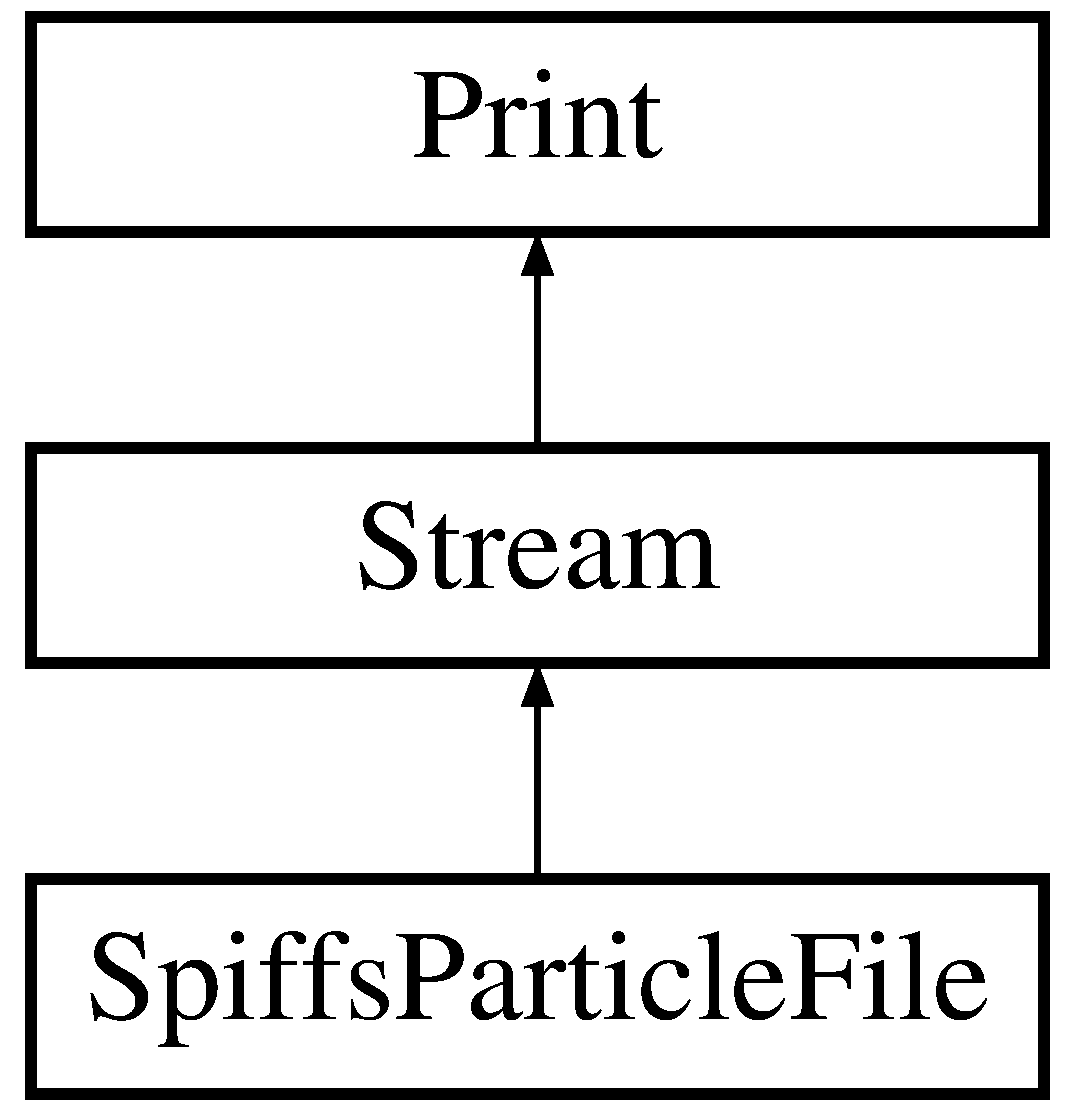
\includegraphics[height=3.000000cm]{class_print}
\end{center}
\end{figure}
\subsection*{Public Member Functions}
\begin{DoxyCompactItemize}
\item 
\mbox{\Hypertarget{class_print_a88a4a829fb5d589efb43955ad0cbddcc}\label{class_print_a88a4a829fb5d589efb43955ad0cbddcc}} 
int \mbox{\hyperlink{class_print_a88a4a829fb5d589efb43955ad0cbddcc}{get\+Write\+Error}} ()
\begin{DoxyCompactList}\small\item\em Return the last error code. \end{DoxyCompactList}\item 
\mbox{\Hypertarget{class_print_aec9ecf84cc6d9087a650def3cefc459e}\label{class_print_aec9ecf84cc6d9087a650def3cefc459e}} 
void \mbox{\hyperlink{class_print_aec9ecf84cc6d9087a650def3cefc459e}{clear\+Write\+Error}} ()
\begin{DoxyCompactList}\small\item\em Clear the last error code. \end{DoxyCompactList}\item 
\mbox{\Hypertarget{class_print_a5be30d49adae2406a270c29ba9a3e0a3}\label{class_print_a5be30d49adae2406a270c29ba9a3e0a3}} 
virtual size\+\_\+t \mbox{\hyperlink{class_print_a5be30d49adae2406a270c29ba9a3e0a3}{write}} (uint8\+\_\+t)=0
\begin{DoxyCompactList}\small\item\em Write a single byte to the stream or file. \end{DoxyCompactList}\item 
size\+\_\+t \mbox{\hyperlink{class_print_a5b40e0e9cab1f2fe5bb0cb22ffe5adda}{write}} (const char $\ast$str)
\begin{DoxyCompactList}\small\item\em Write a null-\/terminated c-\/string the stream or file. \end{DoxyCompactList}\item 
virtual size\+\_\+t \mbox{\hyperlink{class_print_a88864e109589a5be9b0f5ba1327f8421}{write}} (const uint8\+\_\+t $\ast$buffer, size\+\_\+t size)
\begin{DoxyCompactList}\small\item\em Write a bytes specified by a buffer and length to the stream or file. \end{DoxyCompactList}\item 
\mbox{\Hypertarget{class_print_acfe80773011eb17dfb52c2fba517a093}\label{class_print_acfe80773011eb17dfb52c2fba517a093}} 
size\+\_\+t \mbox{\hyperlink{class_print_acfe80773011eb17dfb52c2fba517a093}{print}} (const char\mbox{[}$\,$\mbox{]})
\begin{DoxyCompactList}\small\item\em \mbox{\hyperlink{class_print}{Print}} a null-\/terminated array of char variables (a c-\/string) to the stream or file. \end{DoxyCompactList}\item 
\mbox{\Hypertarget{class_print_a1e411d07a8ffec5faf7ce485bac0f029}\label{class_print_a1e411d07a8ffec5faf7ce485bac0f029}} 
size\+\_\+t \mbox{\hyperlink{class_print_a1e411d07a8ffec5faf7ce485bac0f029}{print}} (char)
\begin{DoxyCompactList}\small\item\em \mbox{\hyperlink{class_print}{Print}} a single character to the stream or file. \end{DoxyCompactList}\item 
size\+\_\+t \mbox{\hyperlink{class_print_ae35481e77567618140cd58d8b96d3747}{print}} (unsigned char value, int base=D\+EC)
\begin{DoxyCompactList}\small\item\em \mbox{\hyperlink{class_print}{Print}} an unsigned char (byte value) in the specified base to the stream or file. \end{DoxyCompactList}\item 
size\+\_\+t \mbox{\hyperlink{class_print_aa28ddbde83b14df73b41c919ecc4478f}{print}} (int value, int base=D\+EC)
\begin{DoxyCompactList}\small\item\em \mbox{\hyperlink{class_print}{Print}} an int the specified base to the stream or file. \end{DoxyCompactList}\item 
size\+\_\+t \mbox{\hyperlink{class_print_afcd7d3a184df961a502643e4fb638c52}{print}} (unsigned int value, int base=D\+EC)
\begin{DoxyCompactList}\small\item\em \mbox{\hyperlink{class_print}{Print}} an unsigned int the specified base to the stream or file. \end{DoxyCompactList}\item 
size\+\_\+t \mbox{\hyperlink{class_print_a0c663ac015ebc037ea044ba2e2cf2947}{print}} (long value, int base=D\+EC)
\begin{DoxyCompactList}\small\item\em \mbox{\hyperlink{class_print}{Print}} a long the specified base to the stream or file. \end{DoxyCompactList}\item 
size\+\_\+t \mbox{\hyperlink{class_print_acb8c6dcd4339b024436002aa9a6f4be2}{print}} (unsigned long value, int base=D\+EC)
\begin{DoxyCompactList}\small\item\em \mbox{\hyperlink{class_print}{Print}} a unsigned long the specified base to the stream or file. \end{DoxyCompactList}\item 
size\+\_\+t \mbox{\hyperlink{class_print_ad89472bdb6539423a42d350beec02ff4}{print}} (double value, int dec=2)
\begin{DoxyCompactList}\small\item\em \mbox{\hyperlink{class_print}{Print}} a double floating point value to the stream or file. \end{DoxyCompactList}\item 
\mbox{\Hypertarget{class_print_a901b0f06ae34aab31b8fbb4298f0596e}\label{class_print_a901b0f06ae34aab31b8fbb4298f0596e}} 
size\+\_\+t \mbox{\hyperlink{class_print_a901b0f06ae34aab31b8fbb4298f0596e}{print}} (const Printable \&)
\begin{DoxyCompactList}\small\item\em \mbox{\hyperlink{class_print}{Print}} an object derived from Printable to the stream or file. \end{DoxyCompactList}\item 
\mbox{\Hypertarget{class_print_ad337ce3f7977411b7d34d47a51e5737e}\label{class_print_ad337ce3f7977411b7d34d47a51e5737e}} 
size\+\_\+t \mbox{\hyperlink{class_print_ad337ce3f7977411b7d34d47a51e5737e}{println}} (const char\mbox{[}$\,$\mbox{]})
\begin{DoxyCompactList}\small\item\em \mbox{\hyperlink{class_print}{Print}} a null-\/terminated array of char variables (a c-\/string) plus a C\+R\+LF end-\/of-\/line terminator to the stream or file. \end{DoxyCompactList}\item 
\mbox{\Hypertarget{class_print_a80fdd92db4b396062586bcb3e08d3835}\label{class_print_a80fdd92db4b396062586bcb3e08d3835}} 
size\+\_\+t \mbox{\hyperlink{class_print_a80fdd92db4b396062586bcb3e08d3835}{println}} (char value)
\begin{DoxyCompactList}\small\item\em \mbox{\hyperlink{class_print}{Print}} a single character plus a C\+R\+LF end-\/of-\/line terminator to the stream or file. \end{DoxyCompactList}\item 
size\+\_\+t \mbox{\hyperlink{class_print_a000b3fd5b723cb6c7db0d3231a9ef2f8}{println}} (unsigned char value, int base=D\+EC)
\begin{DoxyCompactList}\small\item\em \mbox{\hyperlink{class_print}{Print}} an unsigned char (byte value) in the specified base plus a C\+R\+LF end-\/of-\/line terminator to the stream or file. \end{DoxyCompactList}\item 
size\+\_\+t \mbox{\hyperlink{class_print_a82aa91bbd859f28a0a3b4869e5bfcadd}{println}} (int value, int base=D\+EC)
\begin{DoxyCompactList}\small\item\em \mbox{\hyperlink{class_print}{Print}} an int the specified base to plus a C\+R\+LF end-\/of-\/line terminator the stream or file. \end{DoxyCompactList}\item 
size\+\_\+t \mbox{\hyperlink{class_print_a2608232c1f10f654111ff447de16d60b}{println}} (unsigned int value, int base=D\+EC)
\begin{DoxyCompactList}\small\item\em \mbox{\hyperlink{class_print}{Print}} an unsigned int the specified base plus a C\+R\+LF end-\/of-\/line terminator to the stream or file. \end{DoxyCompactList}\item 
size\+\_\+t \mbox{\hyperlink{class_print_a82bbe59b28440c29e55ff3597eb45376}{println}} (long value, int base=D\+EC)
\begin{DoxyCompactList}\small\item\em \mbox{\hyperlink{class_print}{Print}} a long the specified base plus a C\+R\+LF end-\/of-\/line terminator to the stream or file. \end{DoxyCompactList}\item 
size\+\_\+t \mbox{\hyperlink{class_print_afa936d7e8dd329d9162f2cd28f42681e}{println}} (unsigned long value, int base=D\+EC)
\begin{DoxyCompactList}\small\item\em \mbox{\hyperlink{class_print}{Print}} a unsigned long the specified base plus a C\+R\+LF end-\/of-\/line terminator to the stream or file. \end{DoxyCompactList}\item 
size\+\_\+t \mbox{\hyperlink{class_print_a178b90baf9f74f0945f5c64aafec59ea}{println}} (double value, int dec=2)
\begin{DoxyCompactList}\small\item\em \mbox{\hyperlink{class_print}{Print}} a double floating point value plus a C\+R\+LF end-\/of-\/line terminator to the stream or file. \end{DoxyCompactList}\item 
\mbox{\Hypertarget{class_print_a20f9e104153b62e720c9b4c348b44f00}\label{class_print_a20f9e104153b62e720c9b4c348b44f00}} 
size\+\_\+t \mbox{\hyperlink{class_print_a20f9e104153b62e720c9b4c348b44f00}{println}} (const Printable \&)
\begin{DoxyCompactList}\small\item\em \mbox{\hyperlink{class_print}{Print}} an object derived from Printable plus a C\+R\+LF end-\/of-\/line terminator to the stream or file. \end{DoxyCompactList}\item 
\mbox{\Hypertarget{class_print_a169b128f9e22f0c15883768f580541a2}\label{class_print_a169b128f9e22f0c15883768f580541a2}} 
size\+\_\+t \mbox{\hyperlink{class_print_a169b128f9e22f0c15883768f580541a2}{println}} (void)
\begin{DoxyCompactList}\small\item\em \mbox{\hyperlink{class_print}{Print}} a C\+R\+LF end-\/of-\/line terminator to the stream or file. \end{DoxyCompactList}\item 
{\footnotesize template$<$typename... Args$>$ }\\size\+\_\+t \mbox{\hyperlink{class_print_a08a461c9fee5fd8f5795d6e9f61e3d5b}{printf}} (const char $\ast$format, Args... args)
\begin{DoxyCompactList}\small\item\em \mbox{\hyperlink{class_print}{Print}} using printf-\/style formatting to the stream or file. \end{DoxyCompactList}\item 
{\footnotesize template$<$typename... Args$>$ }\\size\+\_\+t \mbox{\hyperlink{class_print_afa41aa5211c54b7b4d79b9286880c337}{printlnf}} (const char $\ast$format, Args... args)
\begin{DoxyCompactList}\small\item\em \mbox{\hyperlink{class_print}{Print}} using printf-\/style formatting plus a C\+R\+LF end-\/of-\/line terminator to the stream or file. \end{DoxyCompactList}\end{DoxyCompactItemize}


\subsection{Detailed Description}
Class for printing to a stream or file. 

Various classes include serial, T\+CP network streams, and files inherit from this and can use these methods. 

\subsection{Member Function Documentation}
\mbox{\Hypertarget{class_print_ae35481e77567618140cd58d8b96d3747}\label{class_print_ae35481e77567618140cd58d8b96d3747}} 
\index{Print@{Print}!print@{print}}
\index{print@{print}!Print@{Print}}
\subsubsection{\texorpdfstring{print()}{print()}\hspace{0.1cm}{\footnotesize\ttfamily [1/6]}}
{\footnotesize\ttfamily size\+\_\+t Print\+::print (\begin{DoxyParamCaption}\item[{unsigned char}]{value,  }\item[{int}]{base = {\ttfamily DEC} }\end{DoxyParamCaption})}



\mbox{\hyperlink{class_print}{Print}} an unsigned char (byte value) in the specified base to the stream or file. 


\begin{DoxyParams}{Parameters}
{\em value} & The value to print \\
\hline
{\em base} & The base to print. Default is D\+EC (decimal). Other values are H\+EX (hexadecimal), O\+CT (octal), and B\+IN (binary). \\
\hline
\end{DoxyParams}
\mbox{\Hypertarget{class_print_aa28ddbde83b14df73b41c919ecc4478f}\label{class_print_aa28ddbde83b14df73b41c919ecc4478f}} 
\index{Print@{Print}!print@{print}}
\index{print@{print}!Print@{Print}}
\subsubsection{\texorpdfstring{print()}{print()}\hspace{0.1cm}{\footnotesize\ttfamily [2/6]}}
{\footnotesize\ttfamily size\+\_\+t Print\+::print (\begin{DoxyParamCaption}\item[{int}]{value,  }\item[{int}]{base = {\ttfamily DEC} }\end{DoxyParamCaption})}



\mbox{\hyperlink{class_print}{Print}} an int the specified base to the stream or file. 


\begin{DoxyParams}{Parameters}
{\em value} & The value to print \\
\hline
{\em base} & The base to print. Default is D\+EC (decimal). Other values are H\+EX (hexadecimal), O\+CT (octal), and B\+IN (binary). \\
\hline
\end{DoxyParams}
\mbox{\Hypertarget{class_print_afcd7d3a184df961a502643e4fb638c52}\label{class_print_afcd7d3a184df961a502643e4fb638c52}} 
\index{Print@{Print}!print@{print}}
\index{print@{print}!Print@{Print}}
\subsubsection{\texorpdfstring{print()}{print()}\hspace{0.1cm}{\footnotesize\ttfamily [3/6]}}
{\footnotesize\ttfamily size\+\_\+t Print\+::print (\begin{DoxyParamCaption}\item[{unsigned int}]{value,  }\item[{int}]{base = {\ttfamily DEC} }\end{DoxyParamCaption})}



\mbox{\hyperlink{class_print}{Print}} an unsigned int the specified base to the stream or file. 


\begin{DoxyParams}{Parameters}
{\em value} & The value to print \\
\hline
{\em base} & The base to print. Default is D\+EC (decimal). Other values are H\+EX (hexadecimal), O\+CT (octal), and B\+IN (binary). \\
\hline
\end{DoxyParams}
\mbox{\Hypertarget{class_print_a0c663ac015ebc037ea044ba2e2cf2947}\label{class_print_a0c663ac015ebc037ea044ba2e2cf2947}} 
\index{Print@{Print}!print@{print}}
\index{print@{print}!Print@{Print}}
\subsubsection{\texorpdfstring{print()}{print()}\hspace{0.1cm}{\footnotesize\ttfamily [4/6]}}
{\footnotesize\ttfamily size\+\_\+t Print\+::print (\begin{DoxyParamCaption}\item[{long}]{value,  }\item[{int}]{base = {\ttfamily DEC} }\end{DoxyParamCaption})}



\mbox{\hyperlink{class_print}{Print}} a long the specified base to the stream or file. 


\begin{DoxyParams}{Parameters}
{\em value} & The value to print \\
\hline
{\em base} & The base to print. Default is D\+EC (decimal). Other values are H\+EX (hexadecimal), O\+CT (octal), and B\+IN (binary). \\
\hline
\end{DoxyParams}
\mbox{\Hypertarget{class_print_acb8c6dcd4339b024436002aa9a6f4be2}\label{class_print_acb8c6dcd4339b024436002aa9a6f4be2}} 
\index{Print@{Print}!print@{print}}
\index{print@{print}!Print@{Print}}
\subsubsection{\texorpdfstring{print()}{print()}\hspace{0.1cm}{\footnotesize\ttfamily [5/6]}}
{\footnotesize\ttfamily size\+\_\+t Print\+::print (\begin{DoxyParamCaption}\item[{unsigned long}]{value,  }\item[{int}]{base = {\ttfamily DEC} }\end{DoxyParamCaption})}



\mbox{\hyperlink{class_print}{Print}} a unsigned long the specified base to the stream or file. 


\begin{DoxyParams}{Parameters}
{\em value} & The value to print \\
\hline
{\em base} & The base to print. Default is D\+EC (decimal). Other values are H\+EX (hexadecimal), O\+CT (octal), and B\+IN (binary). \\
\hline
\end{DoxyParams}
\mbox{\Hypertarget{class_print_ad89472bdb6539423a42d350beec02ff4}\label{class_print_ad89472bdb6539423a42d350beec02ff4}} 
\index{Print@{Print}!print@{print}}
\index{print@{print}!Print@{Print}}
\subsubsection{\texorpdfstring{print()}{print()}\hspace{0.1cm}{\footnotesize\ttfamily [6/6]}}
{\footnotesize\ttfamily size\+\_\+t Print\+::print (\begin{DoxyParamCaption}\item[{double}]{value,  }\item[{int}]{dec = {\ttfamily 2} }\end{DoxyParamCaption})}



\mbox{\hyperlink{class_print}{Print}} a double floating point value to the stream or file. 


\begin{DoxyParams}{Parameters}
{\em value} & The value to print \\
\hline
{\em dec} & The number of decimal places to include for the fractional part. Default\+: 2 \\
\hline
\end{DoxyParams}
\mbox{\Hypertarget{class_print_a08a461c9fee5fd8f5795d6e9f61e3d5b}\label{class_print_a08a461c9fee5fd8f5795d6e9f61e3d5b}} 
\index{Print@{Print}!printf@{printf}}
\index{printf@{printf}!Print@{Print}}
\subsubsection{\texorpdfstring{printf()}{printf()}}
{\footnotesize\ttfamily template$<$typename... Args$>$ \\
size\+\_\+t Print\+::printf (\begin{DoxyParamCaption}\item[{const char $\ast$}]{format,  }\item[{Args...}]{args }\end{DoxyParamCaption})\hspace{0.3cm}{\ttfamily [inline]}}



\mbox{\hyperlink{class_print}{Print}} using printf-\/style formatting to the stream or file. 


\begin{DoxyParams}{Parameters}
{\em format} & printf-\/style formatting string\\
\hline
{\em args} & variable arguments \\
\hline
\end{DoxyParams}
\mbox{\Hypertarget{class_print_a000b3fd5b723cb6c7db0d3231a9ef2f8}\label{class_print_a000b3fd5b723cb6c7db0d3231a9ef2f8}} 
\index{Print@{Print}!println@{println}}
\index{println@{println}!Print@{Print}}
\subsubsection{\texorpdfstring{println()}{println()}\hspace{0.1cm}{\footnotesize\ttfamily [1/6]}}
{\footnotesize\ttfamily size\+\_\+t Print\+::println (\begin{DoxyParamCaption}\item[{unsigned char}]{value,  }\item[{int}]{base = {\ttfamily DEC} }\end{DoxyParamCaption})}



\mbox{\hyperlink{class_print}{Print}} an unsigned char (byte value) in the specified base plus a C\+R\+LF end-\/of-\/line terminator to the stream or file. 


\begin{DoxyParams}{Parameters}
{\em value} & The value to print \\
\hline
{\em base} & The base to print. Default is D\+EC (decimal). Other values are H\+EX (hexadecimal), O\+CT (octal), and B\+IN (binary). \\
\hline
\end{DoxyParams}
\mbox{\Hypertarget{class_print_a82aa91bbd859f28a0a3b4869e5bfcadd}\label{class_print_a82aa91bbd859f28a0a3b4869e5bfcadd}} 
\index{Print@{Print}!println@{println}}
\index{println@{println}!Print@{Print}}
\subsubsection{\texorpdfstring{println()}{println()}\hspace{0.1cm}{\footnotesize\ttfamily [2/6]}}
{\footnotesize\ttfamily size\+\_\+t Print\+::println (\begin{DoxyParamCaption}\item[{int}]{value,  }\item[{int}]{base = {\ttfamily DEC} }\end{DoxyParamCaption})}



\mbox{\hyperlink{class_print}{Print}} an int the specified base to plus a C\+R\+LF end-\/of-\/line terminator the stream or file. 


\begin{DoxyParams}{Parameters}
{\em value} & The value to print \\
\hline
{\em base} & The base to print. Default is D\+EC (decimal). Other values are H\+EX (hexadecimal), O\+CT (octal), and B\+IN (binary). \\
\hline
\end{DoxyParams}
\mbox{\Hypertarget{class_print_a2608232c1f10f654111ff447de16d60b}\label{class_print_a2608232c1f10f654111ff447de16d60b}} 
\index{Print@{Print}!println@{println}}
\index{println@{println}!Print@{Print}}
\subsubsection{\texorpdfstring{println()}{println()}\hspace{0.1cm}{\footnotesize\ttfamily [3/6]}}
{\footnotesize\ttfamily size\+\_\+t Print\+::println (\begin{DoxyParamCaption}\item[{unsigned int}]{value,  }\item[{int}]{base = {\ttfamily DEC} }\end{DoxyParamCaption})}



\mbox{\hyperlink{class_print}{Print}} an unsigned int the specified base plus a C\+R\+LF end-\/of-\/line terminator to the stream or file. 


\begin{DoxyParams}{Parameters}
{\em value} & The value to print \\
\hline
{\em base} & The base to print. Default is D\+EC (decimal). Other values are H\+EX (hexadecimal), O\+CT (octal), and B\+IN (binary). \\
\hline
\end{DoxyParams}
\mbox{\Hypertarget{class_print_a82bbe59b28440c29e55ff3597eb45376}\label{class_print_a82bbe59b28440c29e55ff3597eb45376}} 
\index{Print@{Print}!println@{println}}
\index{println@{println}!Print@{Print}}
\subsubsection{\texorpdfstring{println()}{println()}\hspace{0.1cm}{\footnotesize\ttfamily [4/6]}}
{\footnotesize\ttfamily size\+\_\+t Print\+::println (\begin{DoxyParamCaption}\item[{long}]{value,  }\item[{int}]{base = {\ttfamily DEC} }\end{DoxyParamCaption})}



\mbox{\hyperlink{class_print}{Print}} a long the specified base plus a C\+R\+LF end-\/of-\/line terminator to the stream or file. 


\begin{DoxyParams}{Parameters}
{\em value} & The value to print \\
\hline
{\em base} & The base to print. Default is D\+EC (decimal). Other values are H\+EX (hexadecimal), O\+CT (octal), and B\+IN (binary). \\
\hline
\end{DoxyParams}
\mbox{\Hypertarget{class_print_afa936d7e8dd329d9162f2cd28f42681e}\label{class_print_afa936d7e8dd329d9162f2cd28f42681e}} 
\index{Print@{Print}!println@{println}}
\index{println@{println}!Print@{Print}}
\subsubsection{\texorpdfstring{println()}{println()}\hspace{0.1cm}{\footnotesize\ttfamily [5/6]}}
{\footnotesize\ttfamily size\+\_\+t Print\+::println (\begin{DoxyParamCaption}\item[{unsigned long}]{value,  }\item[{int}]{base = {\ttfamily DEC} }\end{DoxyParamCaption})}



\mbox{\hyperlink{class_print}{Print}} a unsigned long the specified base plus a C\+R\+LF end-\/of-\/line terminator to the stream or file. 


\begin{DoxyParams}{Parameters}
{\em value} & The value to print \\
\hline
{\em base} & The base to print. Default is D\+EC (decimal). Other values are H\+EX (hexadecimal), O\+CT (octal), and B\+IN (binary). \\
\hline
\end{DoxyParams}
\mbox{\Hypertarget{class_print_a178b90baf9f74f0945f5c64aafec59ea}\label{class_print_a178b90baf9f74f0945f5c64aafec59ea}} 
\index{Print@{Print}!println@{println}}
\index{println@{println}!Print@{Print}}
\subsubsection{\texorpdfstring{println()}{println()}\hspace{0.1cm}{\footnotesize\ttfamily [6/6]}}
{\footnotesize\ttfamily size\+\_\+t Print\+::println (\begin{DoxyParamCaption}\item[{double}]{value,  }\item[{int}]{dec = {\ttfamily 2} }\end{DoxyParamCaption})}



\mbox{\hyperlink{class_print}{Print}} a double floating point value plus a C\+R\+LF end-\/of-\/line terminator to the stream or file. 


\begin{DoxyParams}{Parameters}
{\em value} & The value to print \\
\hline
{\em dec} & The number of decimal places to include for the fractional part. Default\+: 2 \\
\hline
\end{DoxyParams}
\mbox{\Hypertarget{class_print_afa41aa5211c54b7b4d79b9286880c337}\label{class_print_afa41aa5211c54b7b4d79b9286880c337}} 
\index{Print@{Print}!printlnf@{printlnf}}
\index{printlnf@{printlnf}!Print@{Print}}
\subsubsection{\texorpdfstring{printlnf()}{printlnf()}}
{\footnotesize\ttfamily template$<$typename... Args$>$ \\
size\+\_\+t Print\+::printlnf (\begin{DoxyParamCaption}\item[{const char $\ast$}]{format,  }\item[{Args...}]{args }\end{DoxyParamCaption})\hspace{0.3cm}{\ttfamily [inline]}}



\mbox{\hyperlink{class_print}{Print}} using printf-\/style formatting plus a C\+R\+LF end-\/of-\/line terminator to the stream or file. 


\begin{DoxyParams}{Parameters}
{\em format} & printf-\/style formatting string\\
\hline
{\em args} & variable arguments \\
\hline
\end{DoxyParams}
\mbox{\Hypertarget{class_print_a5b40e0e9cab1f2fe5bb0cb22ffe5adda}\label{class_print_a5b40e0e9cab1f2fe5bb0cb22ffe5adda}} 
\index{Print@{Print}!write@{write}}
\index{write@{write}!Print@{Print}}
\subsubsection{\texorpdfstring{write()}{write()}\hspace{0.1cm}{\footnotesize\ttfamily [1/2]}}
{\footnotesize\ttfamily size\+\_\+t Print\+::write (\begin{DoxyParamCaption}\item[{const char $\ast$}]{str }\end{DoxyParamCaption})\hspace{0.3cm}{\ttfamily [inline]}}



Write a null-\/terminated c-\/string the stream or file. 


\begin{DoxyParams}{Parameters}
{\em str} & point to a null-\/terminated c-\/string \\
\hline
\end{DoxyParams}
\mbox{\Hypertarget{class_print_a88864e109589a5be9b0f5ba1327f8421}\label{class_print_a88864e109589a5be9b0f5ba1327f8421}} 
\index{Print@{Print}!write@{write}}
\index{write@{write}!Print@{Print}}
\subsubsection{\texorpdfstring{write()}{write()}\hspace{0.1cm}{\footnotesize\ttfamily [2/2]}}
{\footnotesize\ttfamily virtual size\+\_\+t Print\+::write (\begin{DoxyParamCaption}\item[{const uint8\+\_\+t $\ast$}]{buffer,  }\item[{size\+\_\+t}]{size }\end{DoxyParamCaption})\hspace{0.3cm}{\ttfamily [virtual]}}



Write a bytes specified by a buffer and length to the stream or file. 


\begin{DoxyParams}{Parameters}
{\em buffer} & pointer to the buffer \\
\hline
{\em size} & size in bytes \\
\hline
\end{DoxyParams}


Reimplemented in \mbox{\hyperlink{class_spiffs_particle_file_ada3fa1782a929e32adab1c161f9d5eeb}{Spiffs\+Particle\+File}}.



The documentation for this class was generated from the following file\+:\begin{DoxyCompactItemize}
\item 
docs/src/\mbox{\hyperlink{spark__wiring__print_8h}{spark\+\_\+wiring\+\_\+print.\+h}}\end{DoxyCompactItemize}

\hypertarget{structspiffs__config}{}\section{spiffs\+\_\+config Struct Reference}
\label{structspiffs__config}\index{spiffs\+\_\+config@{spiffs\+\_\+config}}
\subsection*{Data Fields}
\begin{DoxyCompactItemize}
\item 
\mbox{\Hypertarget{structspiffs__config_a2d2cc2d17896ba4f5e78c524cd7da76b}\label{structspiffs__config_a2d2cc2d17896ba4f5e78c524cd7da76b}} 
spiffs\+\_\+read {\bfseries hal\+\_\+read\+\_\+f}
\item 
\mbox{\Hypertarget{structspiffs__config_ab9402faf21097e938cb86b70efab38b4}\label{structspiffs__config_ab9402faf21097e938cb86b70efab38b4}} 
spiffs\+\_\+write {\bfseries hal\+\_\+write\+\_\+f}
\item 
\mbox{\Hypertarget{structspiffs__config_a86af9c6671604e9c6e08cfe6c3fdfaeb}\label{structspiffs__config_a86af9c6671604e9c6e08cfe6c3fdfaeb}} 
spiffs\+\_\+erase {\bfseries hal\+\_\+erase\+\_\+f}
\item 
\mbox{\Hypertarget{structspiffs__config_ad1746f2435254dd38ebdbf167a3289e0}\label{structspiffs__config_ad1746f2435254dd38ebdbf167a3289e0}} 
u32\+\_\+t {\bfseries phys\+\_\+size}
\item 
\mbox{\Hypertarget{structspiffs__config_ad14f81b04bcc96bb09909015e06a5b3f}\label{structspiffs__config_ad14f81b04bcc96bb09909015e06a5b3f}} 
u32\+\_\+t {\bfseries phys\+\_\+addr}
\item 
\mbox{\Hypertarget{structspiffs__config_a5d33e08b152880f482c976f897a1632f}\label{structspiffs__config_a5d33e08b152880f482c976f897a1632f}} 
u32\+\_\+t {\bfseries phys\+\_\+erase\+\_\+block}
\item 
\mbox{\Hypertarget{structspiffs__config_afda08e08a059b922706188f6f2c557ac}\label{structspiffs__config_afda08e08a059b922706188f6f2c557ac}} 
u32\+\_\+t {\bfseries log\+\_\+block\+\_\+size}
\item 
\mbox{\Hypertarget{structspiffs__config_a2525c28d372c9d46152b9997972c25fd}\label{structspiffs__config_a2525c28d372c9d46152b9997972c25fd}} 
u32\+\_\+t {\bfseries log\+\_\+page\+\_\+size}
\end{DoxyCompactItemize}


The documentation for this struct was generated from the following file\+:\begin{DoxyCompactItemize}
\item 
src/spiffs.\+h\end{DoxyCompactItemize}

\hypertarget{structspiffs___d_i_r}{}\section{spiffs\+\_\+\+D\+IR Struct Reference}
\label{structspiffs___d_i_r}\index{spiffs\+\_\+\+D\+IR@{spiffs\+\_\+\+D\+IR}}
\subsection*{Data Fields}
\begin{DoxyCompactItemize}
\item 
\mbox{\Hypertarget{structspiffs___d_i_r_ad006821d5233083eaf04fa13fae90d88}\label{structspiffs___d_i_r_ad006821d5233083eaf04fa13fae90d88}} 
\mbox{\hyperlink{structspiffs__t}{spiffs}} $\ast$ {\bfseries fs}
\item 
\mbox{\Hypertarget{structspiffs___d_i_r_a822b1a3cdc78d84d377af471cde6cbc0}\label{structspiffs___d_i_r_a822b1a3cdc78d84d377af471cde6cbc0}} 
spiffs\+\_\+block\+\_\+ix {\bfseries block}
\item 
\mbox{\Hypertarget{structspiffs___d_i_r_a14d25754d25e2dab074381fd20395c2e}\label{structspiffs___d_i_r_a14d25754d25e2dab074381fd20395c2e}} 
int {\bfseries entry}
\end{DoxyCompactItemize}


The documentation for this struct was generated from the following file\+:\begin{DoxyCompactItemize}
\item 
src/spiffs.\+h\end{DoxyCompactItemize}

\hypertarget{structspiffs__dirent}{}\section{spiffs\+\_\+dirent Struct Reference}
\label{structspiffs__dirent}\index{spiffs\+\_\+dirent@{spiffs\+\_\+dirent}}
\subsection*{Data Fields}
\begin{DoxyCompactItemize}
\item 
\mbox{\Hypertarget{structspiffs__dirent_adb9c8e8a7c378611c58c02c4a28a9d85}\label{structspiffs__dirent_adb9c8e8a7c378611c58c02c4a28a9d85}} 
spiffs\+\_\+obj\+\_\+id {\bfseries obj\+\_\+id}
\item 
\mbox{\Hypertarget{structspiffs__dirent_abd0b462b485b05eb9ee1703b1ee5beab}\label{structspiffs__dirent_abd0b462b485b05eb9ee1703b1ee5beab}} 
u8\+\_\+t {\bfseries name} \mbox{[}S\+P\+I\+F\+F\+S\+\_\+\+O\+B\+J\+\_\+\+N\+A\+M\+E\+\_\+\+L\+EN\mbox{]}
\item 
\mbox{\Hypertarget{structspiffs__dirent_a38414e80ef79bb9dcf421555e9435f89}\label{structspiffs__dirent_a38414e80ef79bb9dcf421555e9435f89}} 
spiffs\+\_\+obj\+\_\+type {\bfseries type}
\item 
\mbox{\Hypertarget{structspiffs__dirent_a5cbe52f4c2bb069e109857246decc01b}\label{structspiffs__dirent_a5cbe52f4c2bb069e109857246decc01b}} 
u32\+\_\+t {\bfseries size}
\item 
\mbox{\Hypertarget{structspiffs__dirent_af3dd1aaf484385078fa8f171c6c9456d}\label{structspiffs__dirent_af3dd1aaf484385078fa8f171c6c9456d}} 
spiffs\+\_\+page\+\_\+ix {\bfseries pix}
\end{DoxyCompactItemize}


The documentation for this struct was generated from the following file\+:\begin{DoxyCompactItemize}
\item 
src/spiffs.\+h\end{DoxyCompactItemize}

\hypertarget{structspiffs__fd}{}\section{spiffs\+\_\+fd Struct Reference}
\label{structspiffs__fd}\index{spiffs\+\_\+fd@{spiffs\+\_\+fd}}
\subsection*{Data Fields}
\begin{DoxyCompactItemize}
\item 
\mbox{\Hypertarget{structspiffs__fd_aa21f646ac1a63815a78570700fdb8e91}\label{structspiffs__fd_aa21f646ac1a63815a78570700fdb8e91}} 
\mbox{\hyperlink{structspiffs__t}{spiffs}} $\ast$ {\bfseries fs}
\item 
\mbox{\Hypertarget{structspiffs__fd_a5e8476292713fa8e1519e71b032ada35}\label{structspiffs__fd_a5e8476292713fa8e1519e71b032ada35}} 
spiffs\+\_\+file {\bfseries file\+\_\+nbr}
\item 
\mbox{\Hypertarget{structspiffs__fd_a056d0dbea7a38ddda491430b83cca4c6}\label{structspiffs__fd_a056d0dbea7a38ddda491430b83cca4c6}} 
spiffs\+\_\+obj\+\_\+id {\bfseries obj\+\_\+id}
\item 
\mbox{\Hypertarget{structspiffs__fd_afd4f6ecba84676728fc89441de8acec0}\label{structspiffs__fd_afd4f6ecba84676728fc89441de8acec0}} 
u32\+\_\+t {\bfseries size}
\item 
\mbox{\Hypertarget{structspiffs__fd_aff20783acee2a6194396450cd09bf1be}\label{structspiffs__fd_aff20783acee2a6194396450cd09bf1be}} 
spiffs\+\_\+page\+\_\+ix {\bfseries objix\+\_\+hdr\+\_\+pix}
\item 
\mbox{\Hypertarget{structspiffs__fd_a1c6bc0352d42c68802a7f8163ab90ca7}\label{structspiffs__fd_a1c6bc0352d42c68802a7f8163ab90ca7}} 
spiffs\+\_\+page\+\_\+ix {\bfseries cursor\+\_\+objix\+\_\+pix}
\item 
\mbox{\Hypertarget{structspiffs__fd_ac34aa5584f1f378bb63eaf568c1a6b6e}\label{structspiffs__fd_ac34aa5584f1f378bb63eaf568c1a6b6e}} 
spiffs\+\_\+span\+\_\+ix {\bfseries cursor\+\_\+objix\+\_\+spix}
\item 
\mbox{\Hypertarget{structspiffs__fd_a9f017848bfacc49db05c3276e108e3e8}\label{structspiffs__fd_a9f017848bfacc49db05c3276e108e3e8}} 
u32\+\_\+t {\bfseries offset}
\item 
\mbox{\Hypertarget{structspiffs__fd_a761894a2f436b904a8b434f82849ee14}\label{structspiffs__fd_a761894a2f436b904a8b434f82849ee14}} 
u32\+\_\+t {\bfseries fdoffset}
\item 
\mbox{\Hypertarget{structspiffs__fd_a20874e5b8a1ca24d4954400e538d0190}\label{structspiffs__fd_a20874e5b8a1ca24d4954400e538d0190}} 
spiffs\+\_\+flags {\bfseries flags}
\end{DoxyCompactItemize}


The documentation for this struct was generated from the following file\+:\begin{DoxyCompactItemize}
\item 
src/spiffs\+\_\+nucleus.\+h\end{DoxyCompactItemize}

\hypertarget{structspiffs__free__obj__id__state}{}\section{spiffs\+\_\+free\+\_\+obj\+\_\+id\+\_\+state Struct Reference}
\label{structspiffs__free__obj__id__state}\index{spiffs\+\_\+free\+\_\+obj\+\_\+id\+\_\+state@{spiffs\+\_\+free\+\_\+obj\+\_\+id\+\_\+state}}
\subsection*{Data Fields}
\begin{DoxyCompactItemize}
\item 
\mbox{\Hypertarget{structspiffs__free__obj__id__state_a2e23db65adf01c76cfb8dca971dbb565}\label{structspiffs__free__obj__id__state_a2e23db65adf01c76cfb8dca971dbb565}} 
spiffs\+\_\+obj\+\_\+id {\bfseries min\+\_\+obj\+\_\+id}
\item 
\mbox{\Hypertarget{structspiffs__free__obj__id__state_abe3e0e24350052b8c90aed697f23b6f7}\label{structspiffs__free__obj__id__state_abe3e0e24350052b8c90aed697f23b6f7}} 
spiffs\+\_\+obj\+\_\+id {\bfseries max\+\_\+obj\+\_\+id}
\item 
\mbox{\Hypertarget{structspiffs__free__obj__id__state_a4fe8c12907b7d0909f3ab4aa96a2fa42}\label{structspiffs__free__obj__id__state_a4fe8c12907b7d0909f3ab4aa96a2fa42}} 
u32\+\_\+t {\bfseries compaction}
\item 
\mbox{\Hypertarget{structspiffs__free__obj__id__state_a570a92aa2ae0ad99eaa0d15e872ca650}\label{structspiffs__free__obj__id__state_a570a92aa2ae0ad99eaa0d15e872ca650}} 
const u8\+\_\+t $\ast$ {\bfseries conflicting\+\_\+name}
\end{DoxyCompactItemize}


The documentation for this struct was generated from the following file\+:\begin{DoxyCompactItemize}
\item 
src/spiffs\+\_\+nucleus.\+c\end{DoxyCompactItemize}

\hypertarget{structspiffs__gc}{}\section{spiffs\+\_\+gc Struct Reference}
\label{structspiffs__gc}\index{spiffs\+\_\+gc@{spiffs\+\_\+gc}}
\subsection*{Data Fields}
\begin{DoxyCompactItemize}
\item 
\mbox{\Hypertarget{structspiffs__gc_acad948885807fb1c3ea2984a1226c605}\label{structspiffs__gc_acad948885807fb1c3ea2984a1226c605}} 
spiffs\+\_\+gc\+\_\+clean\+\_\+state {\bfseries state}
\item 
\mbox{\Hypertarget{structspiffs__gc_a5ceb2a4237d5656d2a13eb0522c1d52a}\label{structspiffs__gc_a5ceb2a4237d5656d2a13eb0522c1d52a}} 
spiffs\+\_\+obj\+\_\+id {\bfseries cur\+\_\+obj\+\_\+id}
\item 
\mbox{\Hypertarget{structspiffs__gc_a322c5179dc6edb869a20820796a75626}\label{structspiffs__gc_a322c5179dc6edb869a20820796a75626}} 
spiffs\+\_\+span\+\_\+ix {\bfseries cur\+\_\+objix\+\_\+spix}
\item 
\mbox{\Hypertarget{structspiffs__gc_a233b84d5a3761bead2359c77e963e856}\label{structspiffs__gc_a233b84d5a3761bead2359c77e963e856}} 
spiffs\+\_\+page\+\_\+ix {\bfseries cur\+\_\+objix\+\_\+pix}
\item 
\mbox{\Hypertarget{structspiffs__gc_ad0c61b2be67f7a13baa40b714b44984f}\label{structspiffs__gc_ad0c61b2be67f7a13baa40b714b44984f}} 
spiffs\+\_\+page\+\_\+ix {\bfseries cur\+\_\+data\+\_\+pix}
\item 
\mbox{\Hypertarget{structspiffs__gc_ad126f12ddd74c2c933ff546531750252}\label{structspiffs__gc_ad126f12ddd74c2c933ff546531750252}} 
int {\bfseries stored\+\_\+scan\+\_\+entry\+\_\+index}
\item 
\mbox{\Hypertarget{structspiffs__gc_a45a1822bfd5b4252873ed57af1ab667a}\label{structspiffs__gc_a45a1822bfd5b4252873ed57af1ab667a}} 
u8\+\_\+t {\bfseries obj\+\_\+id\+\_\+found}
\end{DoxyCompactItemize}


The documentation for this struct was generated from the following file\+:\begin{DoxyCompactItemize}
\item 
src/spiffs\+\_\+gc.\+c\end{DoxyCompactItemize}

\hypertarget{structspiffs__ix__map}{}\section{spiffs\+\_\+ix\+\_\+map Struct Reference}
\label{structspiffs__ix__map}\index{spiffs\+\_\+ix\+\_\+map@{spiffs\+\_\+ix\+\_\+map}}
\subsection*{Data Fields}
\begin{DoxyCompactItemize}
\item 
\mbox{\Hypertarget{structspiffs__ix__map_a16c980d6657eb2916fcede33bd062004}\label{structspiffs__ix__map_a16c980d6657eb2916fcede33bd062004}} 
spiffs\+\_\+page\+\_\+ix $\ast$ {\bfseries map\+\_\+buf}
\item 
\mbox{\Hypertarget{structspiffs__ix__map_a1a51b6b7e57415165a7c9079894a1a88}\label{structspiffs__ix__map_a1a51b6b7e57415165a7c9079894a1a88}} 
u32\+\_\+t {\bfseries offset}
\item 
\mbox{\Hypertarget{structspiffs__ix__map_a34ffaa7208e9495eaab9f6271f912995}\label{structspiffs__ix__map_a34ffaa7208e9495eaab9f6271f912995}} 
spiffs\+\_\+span\+\_\+ix {\bfseries start\+\_\+spix}
\item 
\mbox{\Hypertarget{structspiffs__ix__map_af82f3c0899fe830e951ef796bee8b348}\label{structspiffs__ix__map_af82f3c0899fe830e951ef796bee8b348}} 
spiffs\+\_\+span\+\_\+ix {\bfseries end\+\_\+spix}
\end{DoxyCompactItemize}


The documentation for this struct was generated from the following file\+:\begin{DoxyCompactItemize}
\item 
src/spiffs.\+h\end{DoxyCompactItemize}

\hypertarget{structspiffs__ix__map__populate__state}{}\section{spiffs\+\_\+ix\+\_\+map\+\_\+populate\+\_\+state Struct Reference}
\label{structspiffs__ix__map__populate__state}\index{spiffs\+\_\+ix\+\_\+map\+\_\+populate\+\_\+state@{spiffs\+\_\+ix\+\_\+map\+\_\+populate\+\_\+state}}
\subsection*{Data Fields}
\begin{DoxyCompactItemize}
\item 
\mbox{\Hypertarget{structspiffs__ix__map__populate__state_a969374b8470b7c3bc58d96b37b540e9b}\label{structspiffs__ix__map__populate__state_a969374b8470b7c3bc58d96b37b540e9b}} 
\mbox{\hyperlink{structspiffs__fd}{spiffs\+\_\+fd}} $\ast$ {\bfseries fd}
\item 
\mbox{\Hypertarget{structspiffs__ix__map__populate__state_a2eaf00d6dda8e323eeb1645785057830}\label{structspiffs__ix__map__populate__state_a2eaf00d6dda8e323eeb1645785057830}} 
u32\+\_\+t {\bfseries remaining\+\_\+objix\+\_\+pages\+\_\+to\+\_\+visit}
\item 
\mbox{\Hypertarget{structspiffs__ix__map__populate__state_aad6e0a21c02c01a12340e33467142a2a}\label{structspiffs__ix__map__populate__state_aad6e0a21c02c01a12340e33467142a2a}} 
spiffs\+\_\+span\+\_\+ix {\bfseries map\+\_\+objix\+\_\+start\+\_\+spix}
\item 
\mbox{\Hypertarget{structspiffs__ix__map__populate__state_af30d4a5056b0f66e9f6af54303832b1a}\label{structspiffs__ix__map__populate__state_af30d4a5056b0f66e9f6af54303832b1a}} 
spiffs\+\_\+span\+\_\+ix {\bfseries map\+\_\+objix\+\_\+end\+\_\+spix}
\end{DoxyCompactItemize}


The documentation for this struct was generated from the following file\+:\begin{DoxyCompactItemize}
\item 
src/spiffs\+\_\+nucleus.\+c\end{DoxyCompactItemize}

\hypertarget{struct_s_p_i_f_f_s___p_a_c_k_e_d}{}\section{S\+P\+I\+F\+F\+S\+\_\+\+P\+A\+C\+K\+ED Struct Reference}
\label{struct_s_p_i_f_f_s___p_a_c_k_e_d}\index{S\+P\+I\+F\+F\+S\+\_\+\+P\+A\+C\+K\+ED@{S\+P\+I\+F\+F\+S\+\_\+\+P\+A\+C\+K\+ED}}
\subsection*{Data Fields}
\begin{DoxyCompactItemize}
\item 
\mbox{\Hypertarget{struct_s_p_i_f_f_s___p_a_c_k_e_d_a610766bf067526f5e600cde282107595}\label{struct_s_p_i_f_f_s___p_a_c_k_e_d_a610766bf067526f5e600cde282107595}} 
spiffs\+\_\+obj\+\_\+id {\bfseries obj\+\_\+id}
\item 
\mbox{\Hypertarget{struct_s_p_i_f_f_s___p_a_c_k_e_d_ad2b494d63964b70b86c66a27eec1e208}\label{struct_s_p_i_f_f_s___p_a_c_k_e_d_ad2b494d63964b70b86c66a27eec1e208}} 
spiffs\+\_\+span\+\_\+ix {\bfseries span\+\_\+ix}
\item 
\mbox{\Hypertarget{struct_s_p_i_f_f_s___p_a_c_k_e_d_a31b830ab36a015849ca211145e2c7ffe}\label{struct_s_p_i_f_f_s___p_a_c_k_e_d_a31b830ab36a015849ca211145e2c7ffe}} 
u8\+\_\+t {\bfseries flags}
\item 
\mbox{\Hypertarget{struct_s_p_i_f_f_s___p_a_c_k_e_d_a57781310180db784f3476def6f7506b7}\label{struct_s_p_i_f_f_s___p_a_c_k_e_d_a57781310180db784f3476def6f7506b7}} 
\mbox{\hyperlink{struct_s_p_i_f_f_s___p_a_c_k_e_d}{spiffs\+\_\+page\+\_\+header}} {\bfseries p\+\_\+hdr}
\item 
\mbox{\Hypertarget{struct_s_p_i_f_f_s___p_a_c_k_e_d_a8b303b250d800a524a9ff51787951f13}\label{struct_s_p_i_f_f_s___p_a_c_k_e_d_a8b303b250d800a524a9ff51787951f13}} 
u8\+\_\+t {\bfseries \+\_\+align} \mbox{[}4 -\/((sizeof(\mbox{\hyperlink{struct_s_p_i_f_f_s___p_a_c_k_e_d}{spiffs\+\_\+page\+\_\+header}})\&3)==0 ? 4 \+:(sizeof(\mbox{\hyperlink{struct_s_p_i_f_f_s___p_a_c_k_e_d}{spiffs\+\_\+page\+\_\+header}})\&3))\mbox{]}
\item 
\mbox{\Hypertarget{struct_s_p_i_f_f_s___p_a_c_k_e_d_aea58187be56f0bb3471c0e7e1c7ba6d5}\label{struct_s_p_i_f_f_s___p_a_c_k_e_d_aea58187be56f0bb3471c0e7e1c7ba6d5}} 
u32\+\_\+t {\bfseries size}
\item 
\mbox{\Hypertarget{struct_s_p_i_f_f_s___p_a_c_k_e_d_a200b626db130ce8dc2a3c64f13063a98}\label{struct_s_p_i_f_f_s___p_a_c_k_e_d_a200b626db130ce8dc2a3c64f13063a98}} 
spiffs\+\_\+obj\+\_\+type {\bfseries type}
\item 
\mbox{\Hypertarget{struct_s_p_i_f_f_s___p_a_c_k_e_d_a3072e1f0b4bf4fd48e546c0a91986cdc}\label{struct_s_p_i_f_f_s___p_a_c_k_e_d_a3072e1f0b4bf4fd48e546c0a91986cdc}} 
u8\+\_\+t {\bfseries name} \mbox{[}S\+P\+I\+F\+F\+S\+\_\+\+O\+B\+J\+\_\+\+N\+A\+M\+E\+\_\+\+L\+EN\mbox{]}
\end{DoxyCompactItemize}


The documentation for this struct was generated from the following file\+:\begin{DoxyCompactItemize}
\item 
src/spiffs\+\_\+nucleus.\+h\end{DoxyCompactItemize}

\hypertarget{structspiffs__stat}{}\section{spiffs\+\_\+stat Struct Reference}
\label{structspiffs__stat}\index{spiffs\+\_\+stat@{spiffs\+\_\+stat}}
\subsection*{Data Fields}
\begin{DoxyCompactItemize}
\item 
\mbox{\Hypertarget{structspiffs__stat_a50f7d3e286b659e09498edf4e17f1daf}\label{structspiffs__stat_a50f7d3e286b659e09498edf4e17f1daf}} 
spiffs\+\_\+obj\+\_\+id {\bfseries obj\+\_\+id}
\item 
\mbox{\Hypertarget{structspiffs__stat_a861b9a64014f77a01b9630278a7c2410}\label{structspiffs__stat_a861b9a64014f77a01b9630278a7c2410}} 
u32\+\_\+t {\bfseries size}
\item 
\mbox{\Hypertarget{structspiffs__stat_ae08c958bb4b22fd9c6d576e1fea23685}\label{structspiffs__stat_ae08c958bb4b22fd9c6d576e1fea23685}} 
spiffs\+\_\+obj\+\_\+type {\bfseries type}
\item 
\mbox{\Hypertarget{structspiffs__stat_a06f9e575229aee0252974423e045fe50}\label{structspiffs__stat_a06f9e575229aee0252974423e045fe50}} 
spiffs\+\_\+page\+\_\+ix {\bfseries pix}
\item 
\mbox{\Hypertarget{structspiffs__stat_a42b32d4cd1868c63f8a8598e5d888a8b}\label{structspiffs__stat_a42b32d4cd1868c63f8a8598e5d888a8b}} 
u8\+\_\+t {\bfseries name} \mbox{[}S\+P\+I\+F\+F\+S\+\_\+\+O\+B\+J\+\_\+\+N\+A\+M\+E\+\_\+\+L\+EN\mbox{]}
\end{DoxyCompactItemize}


The documentation for this struct was generated from the following file\+:\begin{DoxyCompactItemize}
\item 
src/spiffs.\+h\end{DoxyCompactItemize}

\hypertarget{structspiffs__t}{}\section{spiffs\+\_\+t Struct Reference}
\label{structspiffs__t}\index{spiffs\+\_\+t@{spiffs\+\_\+t}}
\subsection*{Data Fields}
\begin{DoxyCompactItemize}
\item 
\mbox{\Hypertarget{structspiffs__t_a7f9247b4b84e6b6a6f3b988fdf83ba99}\label{structspiffs__t_a7f9247b4b84e6b6a6f3b988fdf83ba99}} 
\mbox{\hyperlink{structspiffs__config}{spiffs\+\_\+config}} {\bfseries cfg}
\item 
\mbox{\Hypertarget{structspiffs__t_a8554c5fc24edbd495ed55da15ea172af}\label{structspiffs__t_a8554c5fc24edbd495ed55da15ea172af}} 
u32\+\_\+t {\bfseries block\+\_\+count}
\item 
\mbox{\Hypertarget{structspiffs__t_a0e0cb263ec86272f5a75503d362582c7}\label{structspiffs__t_a0e0cb263ec86272f5a75503d362582c7}} 
spiffs\+\_\+block\+\_\+ix {\bfseries free\+\_\+cursor\+\_\+block\+\_\+ix}
\item 
\mbox{\Hypertarget{structspiffs__t_aa98ef3edf530c19d0847f900720f3499}\label{structspiffs__t_aa98ef3edf530c19d0847f900720f3499}} 
int {\bfseries free\+\_\+cursor\+\_\+obj\+\_\+lu\+\_\+entry}
\item 
\mbox{\Hypertarget{structspiffs__t_ab61206cd5cbcaf8ee4bcd1cdf2fb53ad}\label{structspiffs__t_ab61206cd5cbcaf8ee4bcd1cdf2fb53ad}} 
spiffs\+\_\+block\+\_\+ix {\bfseries cursor\+\_\+block\+\_\+ix}
\item 
\mbox{\Hypertarget{structspiffs__t_aaac9760dde13fbb11ba81871ecee6b7c}\label{structspiffs__t_aaac9760dde13fbb11ba81871ecee6b7c}} 
int {\bfseries cursor\+\_\+obj\+\_\+lu\+\_\+entry}
\item 
\mbox{\Hypertarget{structspiffs__t_aadc62737ea37cf850aa84f7cb0faabb2}\label{structspiffs__t_aadc62737ea37cf850aa84f7cb0faabb2}} 
u8\+\_\+t $\ast$ {\bfseries lu\+\_\+work}
\item 
\mbox{\Hypertarget{structspiffs__t_af48f680e30ac20c12412545af0515201}\label{structspiffs__t_af48f680e30ac20c12412545af0515201}} 
u8\+\_\+t $\ast$ {\bfseries work}
\item 
\mbox{\Hypertarget{structspiffs__t_a4471d7ec110042b1c68cb06311b1daf9}\label{structspiffs__t_a4471d7ec110042b1c68cb06311b1daf9}} 
u8\+\_\+t $\ast$ {\bfseries fd\+\_\+space}
\item 
\mbox{\Hypertarget{structspiffs__t_a1538b44ff998bbc79b59d5adbffeb9dc}\label{structspiffs__t_a1538b44ff998bbc79b59d5adbffeb9dc}} 
u32\+\_\+t {\bfseries fd\+\_\+count}
\item 
\mbox{\Hypertarget{structspiffs__t_a5a2359dde97d3ce7158b0ed37ecca219}\label{structspiffs__t_a5a2359dde97d3ce7158b0ed37ecca219}} 
s32\+\_\+t {\bfseries err\+\_\+code}
\item 
\mbox{\Hypertarget{structspiffs__t_a70cd3e118549e8ec2f20a34725a91a22}\label{structspiffs__t_a70cd3e118549e8ec2f20a34725a91a22}} 
u32\+\_\+t {\bfseries free\+\_\+blocks}
\item 
\mbox{\Hypertarget{structspiffs__t_ac567c1d29a7c3c91c8e9ad480a5f4c59}\label{structspiffs__t_ac567c1d29a7c3c91c8e9ad480a5f4c59}} 
u32\+\_\+t {\bfseries stats\+\_\+p\+\_\+allocated}
\item 
\mbox{\Hypertarget{structspiffs__t_ad261e9db98b460b8e514ef11eaed5220}\label{structspiffs__t_ad261e9db98b460b8e514ef11eaed5220}} 
u32\+\_\+t {\bfseries stats\+\_\+p\+\_\+deleted}
\item 
\mbox{\Hypertarget{structspiffs__t_a57d679557baf30480c0b435461e34f44}\label{structspiffs__t_a57d679557baf30480c0b435461e34f44}} 
u8\+\_\+t {\bfseries cleaning}
\item 
\mbox{\Hypertarget{structspiffs__t_a98c1ac3d41d58deb2f667856901b714f}\label{structspiffs__t_a98c1ac3d41d58deb2f667856901b714f}} 
spiffs\+\_\+obj\+\_\+id {\bfseries max\+\_\+erase\+\_\+count}
\item 
\mbox{\Hypertarget{structspiffs__t_a75d6ec264f80cd51676417ce81a2e0b7}\label{structspiffs__t_a75d6ec264f80cd51676417ce81a2e0b7}} 
u32\+\_\+t {\bfseries stats\+\_\+gc\+\_\+runs}
\item 
\mbox{\Hypertarget{structspiffs__t_a1cbc112befd2dd43441b81f957f6328f}\label{structspiffs__t_a1cbc112befd2dd43441b81f957f6328f}} 
void $\ast$ {\bfseries cache}
\item 
\mbox{\Hypertarget{structspiffs__t_a189fb2ddc2eb3822edf0024369dd302c}\label{structspiffs__t_a189fb2ddc2eb3822edf0024369dd302c}} 
u32\+\_\+t {\bfseries cache\+\_\+size}
\item 
\mbox{\Hypertarget{structspiffs__t_a03c2879c5e9cf780c983a2661eedf56e}\label{structspiffs__t_a03c2879c5e9cf780c983a2661eedf56e}} 
u32\+\_\+t {\bfseries cache\+\_\+hits}
\item 
\mbox{\Hypertarget{structspiffs__t_a1e1ccfa9edf8265df4fd40705336e3a5}\label{structspiffs__t_a1e1ccfa9edf8265df4fd40705336e3a5}} 
u32\+\_\+t {\bfseries cache\+\_\+misses}
\item 
\mbox{\Hypertarget{structspiffs__t_a5eb5f40440f41dfca5e0a3aba520e4b4}\label{structspiffs__t_a5eb5f40440f41dfca5e0a3aba520e4b4}} 
spiffs\+\_\+check\+\_\+callback {\bfseries check\+\_\+cb\+\_\+f}
\item 
\mbox{\Hypertarget{structspiffs__t_ab3da90414142391c3eeeb5905b7eb30b}\label{structspiffs__t_ab3da90414142391c3eeeb5905b7eb30b}} 
spiffs\+\_\+file\+\_\+callback {\bfseries file\+\_\+cb\+\_\+f}
\item 
\mbox{\Hypertarget{structspiffs__t_a542d258081a8be645319ff597cfcedd4}\label{structspiffs__t_a542d258081a8be645319ff597cfcedd4}} 
u8\+\_\+t {\bfseries mounted}
\item 
\mbox{\Hypertarget{structspiffs__t_a00dfd42d670514d50b7a906b75e45a44}\label{structspiffs__t_a00dfd42d670514d50b7a906b75e45a44}} 
void $\ast$ {\bfseries user\+\_\+data}
\item 
\mbox{\Hypertarget{structspiffs__t_acaf98085b60c8f1a916bb4023a2bd3be}\label{structspiffs__t_acaf98085b60c8f1a916bb4023a2bd3be}} 
u32\+\_\+t {\bfseries config\+\_\+magic}
\end{DoxyCompactItemize}


The documentation for this struct was generated from the following file\+:\begin{DoxyCompactItemize}
\item 
src/spiffs.\+h\end{DoxyCompactItemize}

\hypertarget{class_spiffs_particle}{}\section{Spiffs\+Particle Class Reference}
\label{class_spiffs_particle}\index{Spiffs\+Particle@{Spiffs\+Particle}}


C++ wrapper for the S\+P\+I\+F\+FS library for the Particle platform.  




{\ttfamily \#include $<$Spiffs\+Particle\+R\+K.\+h$>$}

\subsection*{Public Member Functions}
\begin{DoxyCompactItemize}
\item 
\mbox{\hyperlink{class_spiffs_particle_a3c3749f4cfae7c6ef1721b84e0964a56}{Spiffs\+Particle}} (Spi\+Flash\+Base \&flash)
\begin{DoxyCompactList}\small\item\em Create a \mbox{\hyperlink{class_spiffs_particle}{Spiffs\+Particle}} file system object. Note that you must mount the file system before using it! \end{DoxyCompactList}\item 
\mbox{\Hypertarget{class_spiffs_particle_a6d58b2716f9ae5b1f5508f4e82e8b6c0}\label{class_spiffs_particle_a6d58b2716f9ae5b1f5508f4e82e8b6c0}} 
\mbox{\hyperlink{class_spiffs_particle}{Spiffs\+Particle}} \& \mbox{\hyperlink{class_spiffs_particle_a6d58b2716f9ae5b1f5508f4e82e8b6c0}{with\+Physical\+Size}} (size\+\_\+t value)
\begin{DoxyCompactList}\small\item\em Sets the size of the flash file system in bytes, relative to the physical start address. \end{DoxyCompactList}\item 
\mbox{\Hypertarget{class_spiffs_particle_a68685e7a6143d550c1f31f0046187426}\label{class_spiffs_particle_a68685e7a6143d550c1f31f0046187426}} 
\mbox{\hyperlink{class_spiffs_particle}{Spiffs\+Particle}} \& \mbox{\hyperlink{class_spiffs_particle_a68685e7a6143d550c1f31f0046187426}{with\+Physical\+Addr}} (size\+\_\+t value)
\begin{DoxyCompactList}\small\item\em Sets the start address in the flash for the file system (default\+: 0) \end{DoxyCompactList}\item 
\mbox{\hyperlink{class_spiffs_particle}{Spiffs\+Particle}} \& \mbox{\hyperlink{class_spiffs_particle_af99c2e3bdc38de7f33761b97a2680cec}{with\+Physical\+Block\+Size}} (size\+\_\+t value)
\begin{DoxyCompactList}\small\item\em Sets the physical block size (default\+: 4096) \end{DoxyCompactList}\item 
\mbox{\hyperlink{class_spiffs_particle}{Spiffs\+Particle}} \& \mbox{\hyperlink{class_spiffs_particle_a9f04b3f3f10aacad3281a8abaf14bac6}{with\+Logical\+Block\+Size}} (size\+\_\+t value)
\begin{DoxyCompactList}\small\item\em Sets the logical block size (default\+: 4096) \end{DoxyCompactList}\item 
\mbox{\hyperlink{class_spiffs_particle}{Spiffs\+Particle}} \& \mbox{\hyperlink{class_spiffs_particle_afb7595fab7db056f0c4594ee5fa2cd48}{with\+Logical\+Page\+Size}} (size\+\_\+t value)
\begin{DoxyCompactList}\small\item\em Sets the logical page size (default\+: 256) \end{DoxyCompactList}\item 
\mbox{\hyperlink{class_spiffs_particle}{Spiffs\+Particle}} \& \mbox{\hyperlink{class_spiffs_particle_a0a88791b69d2711a32b31cef465f2ebe}{with\+Max\+Open\+Files}} (size\+\_\+t value)
\begin{DoxyCompactList}\small\item\em Sets the maximum number of open files (default\+: 4) \end{DoxyCompactList}\item 
\mbox{\hyperlink{class_spiffs_particle}{Spiffs\+Particle}} \& \mbox{\hyperlink{class_spiffs_particle_afc11a0266e8be6fb84ec4735d58281cb}{with\+Cache\+Pages}} (size\+\_\+t value)
\begin{DoxyCompactList}\small\item\em Sets the desired not of cache pages (default\+: 2) \end{DoxyCompactList}\item 
\mbox{\hyperlink{class_spiffs_particle}{Spiffs\+Particle}} \& \mbox{\hyperlink{class_spiffs_particle_a12f034a87b98381d976f81885b66b87a}{with\+Low\+Level\+Debug}} (bool value=true)
\begin{DoxyCompactList}\small\item\em Enable (or disable) low level debug mode. \end{DoxyCompactList}\item 
s32\+\_\+t \mbox{\hyperlink{class_spiffs_particle_a55ce37570d764bb8d00698903211fee8}{mount}} (spiffs\+\_\+check\+\_\+callback callback)
\begin{DoxyCompactList}\small\item\em Mount the file system. \end{DoxyCompactList}\item 
void \mbox{\hyperlink{class_spiffs_particle_a2f1b8abb2c89f1935675240430907f7e}{unmount}} ()
\begin{DoxyCompactList}\small\item\em Unmount the file system. All file handles will be flushed of any cached writes and closed. \end{DoxyCompactList}\item 
s32\+\_\+t \mbox{\hyperlink{class_spiffs_particle_a31500330ba98a081bc7b41f027406bf0}{format}} ()
\begin{DoxyCompactList}\small\item\em Format the file system. \end{DoxyCompactList}\item 
s32\+\_\+t \mbox{\hyperlink{class_spiffs_particle_a377b6476c59d353cedc0c666a3998af4}{erase}} ()
\begin{DoxyCompactList}\small\item\em Erase the sectors used by the file system. Obviously all data will be lost. \end{DoxyCompactList}\item 
s32\+\_\+t \mbox{\hyperlink{class_spiffs_particle_ac2714880969a1b6625de152105e291f5}{creat}} (const char $\ast$path, spiffs\+\_\+mode mode=0777)
\begin{DoxyCompactList}\small\item\em Creates a new file. \end{DoxyCompactList}\item 
spiffs\+\_\+file \mbox{\hyperlink{class_spiffs_particle_a0f13439808a65feb0d307de157598b96}{open}} (const char $\ast$path, spiffs\+\_\+flags flags, spiffs\+\_\+mode mode=0777)
\begin{DoxyCompactList}\small\item\em Opens or creates a file. \end{DoxyCompactList}\item 
\mbox{\hyperlink{class_spiffs_particle_file}{Spiffs\+Particle\+File}} \mbox{\hyperlink{class_spiffs_particle_a19e88cd7e5e352ab0222ac8d5ece430b}{open\+File}} (const char $\ast$path, spiffs\+\_\+flags flags, spiffs\+\_\+mode mode=0777)
\begin{DoxyCompactList}\small\item\em Open a file and return a \mbox{\hyperlink{class_spiffs_particle_file}{Spiffs\+Particle\+File}} object to easily manipulate it using Arduino/\+Wiring style calls. \end{DoxyCompactList}\item 
s32\+\_\+t \mbox{\hyperlink{class_spiffs_particle_a39cfb5a9c5bc2ae9f99a3c5c3bf4e64f}{read}} (spiffs\+\_\+file fh, void $\ast$buf, s32\+\_\+t len)
\begin{DoxyCompactList}\small\item\em Reads from given filehandle. \end{DoxyCompactList}\item 
s32\+\_\+t \mbox{\hyperlink{class_spiffs_particle_a24c19c610c1bc97647d8797ed632a814}{write}} (spiffs\+\_\+file fh, const void $\ast$buf, s32\+\_\+t len)
\begin{DoxyCompactList}\small\item\em Writes to given filehandle. \end{DoxyCompactList}\item 
s32\+\_\+t \mbox{\hyperlink{class_spiffs_particle_a8875ae5bd2177da2b046ac5b6254ec85}{lseek}} (spiffs\+\_\+file fh, s32\+\_\+t offs, int whence)
\begin{DoxyCompactList}\small\item\em Moves the read/write file offset. \end{DoxyCompactList}\item 
s32\+\_\+t \mbox{\hyperlink{class_spiffs_particle_abb6a31d8bb30bbe0816e89f8d15cfd9c}{eof}} (spiffs\+\_\+file fh)
\begin{DoxyCompactList}\small\item\em Check if E\+OF reached. \end{DoxyCompactList}\item 
s32\+\_\+t \mbox{\hyperlink{class_spiffs_particle_a38ddf851ffd2e4ade100114bfe4ca524}{tell}} (spiffs\+\_\+file fh)
\begin{DoxyCompactList}\small\item\em Get position in file. \end{DoxyCompactList}\item 
s32\+\_\+t \mbox{\hyperlink{class_spiffs_particle_a9ee304e19b76f4a68e8f772a92bbd104}{remove}} (const char $\ast$path)
\begin{DoxyCompactList}\small\item\em Removes a file by path. \end{DoxyCompactList}\item 
s32\+\_\+t \mbox{\hyperlink{class_spiffs_particle_a19073c6608c352f93e4a5cff6bb95fb8}{fremove}} (spiffs\+\_\+file fh)
\begin{DoxyCompactList}\small\item\em Removes a file by filehandle. \end{DoxyCompactList}\item 
s32\+\_\+t \mbox{\hyperlink{class_spiffs_particle_af52be85536c06520864bd4918b3fe927}{truncate}} (const char $\ast$path, s32\+\_\+t len)
\begin{DoxyCompactList}\small\item\em Truncate a file by path. \end{DoxyCompactList}\item 
s32\+\_\+t \mbox{\hyperlink{class_spiffs_particle_a9bcb248af1aa3fe66b6a853304765e35}{ftruncate}} (spiffs\+\_\+file fh, s32\+\_\+t len)
\begin{DoxyCompactList}\small\item\em Truncate a file by filehandle. \end{DoxyCompactList}\item 
s32\+\_\+t \mbox{\hyperlink{class_spiffs_particle_a42bc28baf22af229ca371a0a1e2d16a6}{stat}} (const char $\ast$path, \mbox{\hyperlink{structspiffs__stat}{spiffs\+\_\+stat}} $\ast$s)
\begin{DoxyCompactList}\small\item\em Gets file status by path. \end{DoxyCompactList}\item 
s32\+\_\+t \mbox{\hyperlink{class_spiffs_particle_a2ea24c9aded8801cafd373b11dd912d7}{fstat}} (spiffs\+\_\+file fh, \mbox{\hyperlink{structspiffs__stat}{spiffs\+\_\+stat}} $\ast$s)
\begin{DoxyCompactList}\small\item\em Gets file status by filehandle. \end{DoxyCompactList}\item 
s32\+\_\+t \mbox{\hyperlink{class_spiffs_particle_a32b335384933ca63e6f8026759ced629}{fflush}} (spiffs\+\_\+file fh)
\begin{DoxyCompactList}\small\item\em Flushes all pending write operations from cache for given file. \end{DoxyCompactList}\item 
s32\+\_\+t \mbox{\hyperlink{class_spiffs_particle_af9962503f18487131191a5647e32ef2a}{close}} (spiffs\+\_\+file fh)
\begin{DoxyCompactList}\small\item\em Closes a filehandle. If there are pending write operations, these are finalized before closing. \end{DoxyCompactList}\item 
s32\+\_\+t \mbox{\hyperlink{class_spiffs_particle_ad016729fc6bc5560ddb5e5faba089b4f}{rename}} (const char $\ast$old, const char $\ast$new\+Path)
\begin{DoxyCompactList}\small\item\em Renames a file. \end{DoxyCompactList}\item 
\mbox{\Hypertarget{class_spiffs_particle_a638a65a354cc57c4a89fc19af1568cbb}\label{class_spiffs_particle_a638a65a354cc57c4a89fc19af1568cbb}} 
s32\+\_\+t \mbox{\hyperlink{class_spiffs_particle_a638a65a354cc57c4a89fc19af1568cbb}{spiffs\+\_\+errno}} ()
\begin{DoxyCompactList}\small\item\em Returns last error of last file operation. \end{DoxyCompactList}\item 
void \mbox{\hyperlink{class_spiffs_particle_af89255deb61819ea561163652784dcf1}{spiffs\+\_\+clearerr}} ()
\begin{DoxyCompactList}\small\item\em Clears last error. \end{DoxyCompactList}\item 
\mbox{\hyperlink{structspiffs___d_i_r}{spiffs\+\_\+\+D\+IR}} $\ast$ \mbox{\hyperlink{class_spiffs_particle_ae2fdc1f28c8a83a55d9e2b18c734f631}{opendir}} (const char $\ast$name, \mbox{\hyperlink{structspiffs___d_i_r}{spiffs\+\_\+\+D\+IR}} $\ast$d)
\begin{DoxyCompactList}\small\item\em Opens a directory stream corresponding to the given name. The stream is positioned at the first entry in the directory. On hydrogen builds the name argument is ignored as hydrogen builds always correspond to a flat file structure -\/ no directories. \end{DoxyCompactList}\item 
struct \mbox{\hyperlink{structspiffs__dirent}{spiffs\+\_\+dirent}} $\ast$ \mbox{\hyperlink{class_spiffs_particle_a258d05b35100c4b20fdd090810392e56}{readdir}} (\mbox{\hyperlink{structspiffs___d_i_r}{spiffs\+\_\+\+D\+IR}} $\ast$d, struct \mbox{\hyperlink{structspiffs__dirent}{spiffs\+\_\+dirent}} $\ast$e)
\begin{DoxyCompactList}\small\item\em Reads a directory into given spifs\+\_\+dirent struct. \end{DoxyCompactList}\item 
s32\+\_\+t \mbox{\hyperlink{class_spiffs_particle_a6b7038ef799d9c369fac7d52f94032d3}{closedir}} (\mbox{\hyperlink{structspiffs___d_i_r}{spiffs\+\_\+\+D\+IR}} $\ast$d)
\begin{DoxyCompactList}\small\item\em Closes a directory stream. \end{DoxyCompactList}\item 
s32\+\_\+t \mbox{\hyperlink{class_spiffs_particle_a9ca5ff16a1168aef2d0b1aa1b1b9e1e0}{check}} ()
\begin{DoxyCompactList}\small\item\em Runs a consistency check on given filesystem. \end{DoxyCompactList}\item 
s32\+\_\+t \mbox{\hyperlink{class_spiffs_particle_afb2bb434707069b737e54fb342e9831b}{info}} (u32\+\_\+t $\ast$total, u32\+\_\+t $\ast$used)
\begin{DoxyCompactList}\small\item\em Returns number of total bytes available and number of used bytes. This is an estimation, and depends on if there a many files with little data or few files with much data. NB\+: If used number of bytes exceeds total bytes, a S\+P\+I\+F\+F\+S\+\_\+check should run. This indicates a power loss in midst of things. In worst case (repeated powerlosses in mending or gc) you might have to delete some files. \end{DoxyCompactList}\item 
\mbox{\Hypertarget{class_spiffs_particle_a7dca116e5b60e5a46a10a15bdd747ca2}\label{class_spiffs_particle_a7dca116e5b60e5a46a10a15bdd747ca2}} 
bool \mbox{\hyperlink{class_spiffs_particle_a7dca116e5b60e5a46a10a15bdd747ca2}{mounted}} ()
\begin{DoxyCompactList}\small\item\em Returns nonzero if spiffs is mounted, or zero if unmounted. \end{DoxyCompactList}\end{DoxyCompactItemize}
\subsection*{Static Public Member Functions}
\begin{DoxyCompactItemize}
\item 
\mbox{\Hypertarget{class_spiffs_particle_aae0af1b65302b4ef3cd3b95f9239bc12}\label{class_spiffs_particle_aae0af1b65302b4ef3cd3b95f9239bc12}} 
static void \mbox{\hyperlink{class_spiffs_particle_aae0af1b65302b4ef3cd3b95f9239bc12}{info\+Log}} (const char $\ast$fmt,...)
\begin{DoxyCompactList}\small\item\em Used internally to generate an info level log for app.\+spiffs. \end{DoxyCompactList}\item 
\mbox{\Hypertarget{class_spiffs_particle_ab74ae23691bfc91496484cc4cda489d9}\label{class_spiffs_particle_ab74ae23691bfc91496484cc4cda489d9}} 
static void \mbox{\hyperlink{class_spiffs_particle_ab74ae23691bfc91496484cc4cda489d9}{trace\+Log}} (const char $\ast$fmt,...)
\begin{DoxyCompactList}\small\item\em Used internally to generate an trace level log for app.\+spiffs. \end{DoxyCompactList}\end{DoxyCompactItemize}


\subsection{Detailed Description}
C++ wrapper for the S\+P\+I\+F\+FS library for the Particle platform. 

\subsection{Constructor \& Destructor Documentation}
\mbox{\Hypertarget{class_spiffs_particle_a3c3749f4cfae7c6ef1721b84e0964a56}\label{class_spiffs_particle_a3c3749f4cfae7c6ef1721b84e0964a56}} 
\index{Spiffs\+Particle@{Spiffs\+Particle}!Spiffs\+Particle@{Spiffs\+Particle}}
\index{Spiffs\+Particle@{Spiffs\+Particle}!Spiffs\+Particle@{Spiffs\+Particle}}
\subsubsection{\texorpdfstring{Spiffs\+Particle()}{SpiffsParticle()}}
{\footnotesize\ttfamily Spiffs\+Particle\+::\+Spiffs\+Particle (\begin{DoxyParamCaption}\item[{Spi\+Flash\+Base \&}]{flash }\end{DoxyParamCaption})}



Create a \mbox{\hyperlink{class_spiffs_particle}{Spiffs\+Particle}} file system object. Note that you must mount the file system before using it! 

It\textquotesingle{}s safe (and common) to create the \mbox{\hyperlink{class_spiffs_particle}{Spiffs\+Particle}} object as a global variable. 

\subsection{Member Function Documentation}
\mbox{\Hypertarget{class_spiffs_particle_a9ca5ff16a1168aef2d0b1aa1b1b9e1e0}\label{class_spiffs_particle_a9ca5ff16a1168aef2d0b1aa1b1b9e1e0}} 
\index{Spiffs\+Particle@{Spiffs\+Particle}!check@{check}}
\index{check@{check}!Spiffs\+Particle@{Spiffs\+Particle}}
\subsubsection{\texorpdfstring{check()}{check()}}
{\footnotesize\ttfamily s32\+\_\+t Spiffs\+Particle\+::check (\begin{DoxyParamCaption}{ }\end{DoxyParamCaption})\hspace{0.3cm}{\ttfamily [inline]}}



Runs a consistency check on given filesystem. 

This takes a while to run so you probably don\textquotesingle{}t want to do this very often. \mbox{\Hypertarget{class_spiffs_particle_af9962503f18487131191a5647e32ef2a}\label{class_spiffs_particle_af9962503f18487131191a5647e32ef2a}} 
\index{Spiffs\+Particle@{Spiffs\+Particle}!close@{close}}
\index{close@{close}!Spiffs\+Particle@{Spiffs\+Particle}}
\subsubsection{\texorpdfstring{close()}{close()}}
{\footnotesize\ttfamily s32\+\_\+t Spiffs\+Particle\+::close (\begin{DoxyParamCaption}\item[{spiffs\+\_\+file}]{fh }\end{DoxyParamCaption})\hspace{0.3cm}{\ttfamily [inline]}}



Closes a filehandle. If there are pending write operations, these are finalized before closing. 


\begin{DoxyParams}{Parameters}
{\em fh} & the filehandle of the file to close \\
\hline
\end{DoxyParams}
\mbox{\Hypertarget{class_spiffs_particle_a6b7038ef799d9c369fac7d52f94032d3}\label{class_spiffs_particle_a6b7038ef799d9c369fac7d52f94032d3}} 
\index{Spiffs\+Particle@{Spiffs\+Particle}!closedir@{closedir}}
\index{closedir@{closedir}!Spiffs\+Particle@{Spiffs\+Particle}}
\subsubsection{\texorpdfstring{closedir()}{closedir()}}
{\footnotesize\ttfamily s32\+\_\+t Spiffs\+Particle\+::closedir (\begin{DoxyParamCaption}\item[{\mbox{\hyperlink{structspiffs___d_i_r}{spiffs\+\_\+\+D\+IR}} $\ast$}]{d }\end{DoxyParamCaption})\hspace{0.3cm}{\ttfamily [inline]}}



Closes a directory stream. 


\begin{DoxyParams}{Parameters}
{\em d} & the directory stream to close \\
\hline
\end{DoxyParams}
\mbox{\Hypertarget{class_spiffs_particle_ac2714880969a1b6625de152105e291f5}\label{class_spiffs_particle_ac2714880969a1b6625de152105e291f5}} 
\index{Spiffs\+Particle@{Spiffs\+Particle}!creat@{creat}}
\index{creat@{creat}!Spiffs\+Particle@{Spiffs\+Particle}}
\subsubsection{\texorpdfstring{creat()}{creat()}}
{\footnotesize\ttfamily s32\+\_\+t Spiffs\+Particle\+::creat (\begin{DoxyParamCaption}\item[{const char $\ast$}]{path,  }\item[{spiffs\+\_\+mode}]{mode = {\ttfamily 0777} }\end{DoxyParamCaption})\hspace{0.3cm}{\ttfamily [inline]}}



Creates a new file. 


\begin{DoxyParams}{Parameters}
{\em path} & the path of the new file \\
\hline
{\em mode} & ignored, for posix compliance. This is an optional parameter.\\
\hline
\end{DoxyParams}
Note that there are no subdirectories in S\+P\+I\+F\+FS and the maximum filename length is 32. \mbox{\Hypertarget{class_spiffs_particle_abb6a31d8bb30bbe0816e89f8d15cfd9c}\label{class_spiffs_particle_abb6a31d8bb30bbe0816e89f8d15cfd9c}} 
\index{Spiffs\+Particle@{Spiffs\+Particle}!eof@{eof}}
\index{eof@{eof}!Spiffs\+Particle@{Spiffs\+Particle}}
\subsubsection{\texorpdfstring{eof()}{eof()}}
{\footnotesize\ttfamily s32\+\_\+t Spiffs\+Particle\+::eof (\begin{DoxyParamCaption}\item[{spiffs\+\_\+file}]{fh }\end{DoxyParamCaption})\hspace{0.3cm}{\ttfamily [inline]}}



Check if E\+OF reached. 


\begin{DoxyParams}{Parameters}
{\em fh} & the filehandle of the file to check \\
\hline
\end{DoxyParams}
\mbox{\Hypertarget{class_spiffs_particle_a377b6476c59d353cedc0c666a3998af4}\label{class_spiffs_particle_a377b6476c59d353cedc0c666a3998af4}} 
\index{Spiffs\+Particle@{Spiffs\+Particle}!erase@{erase}}
\index{erase@{erase}!Spiffs\+Particle@{Spiffs\+Particle}}
\subsubsection{\texorpdfstring{erase()}{erase()}}
{\footnotesize\ttfamily s32\+\_\+t Spiffs\+Particle\+::erase (\begin{DoxyParamCaption}{ }\end{DoxyParamCaption})}



Erase the sectors used by the file system. Obviously all data will be lost. 

This function returns error S\+P\+I\+F\+F\+S\+\_\+\+E\+R\+R\+\_\+\+M\+O\+U\+N\+T\+ED if the file system is currently mounted; you must unmount it before erasing. \mbox{\Hypertarget{class_spiffs_particle_a32b335384933ca63e6f8026759ced629}\label{class_spiffs_particle_a32b335384933ca63e6f8026759ced629}} 
\index{Spiffs\+Particle@{Spiffs\+Particle}!fflush@{fflush}}
\index{fflush@{fflush}!Spiffs\+Particle@{Spiffs\+Particle}}
\subsubsection{\texorpdfstring{fflush()}{fflush()}}
{\footnotesize\ttfamily s32\+\_\+t Spiffs\+Particle\+::fflush (\begin{DoxyParamCaption}\item[{spiffs\+\_\+file}]{fh }\end{DoxyParamCaption})\hspace{0.3cm}{\ttfamily [inline]}}



Flushes all pending write operations from cache for given file. 


\begin{DoxyParams}{Parameters}
{\em fh} & the filehandle of the file to flush\\
\hline
\end{DoxyParams}
It is not necessary to flush before close; close will flush any data if necessary. \mbox{\Hypertarget{class_spiffs_particle_a31500330ba98a081bc7b41f027406bf0}\label{class_spiffs_particle_a31500330ba98a081bc7b41f027406bf0}} 
\index{Spiffs\+Particle@{Spiffs\+Particle}!format@{format}}
\index{format@{format}!Spiffs\+Particle@{Spiffs\+Particle}}
\subsubsection{\texorpdfstring{format()}{format()}}
{\footnotesize\ttfamily s32\+\_\+t Spiffs\+Particle\+::format (\begin{DoxyParamCaption}{ }\end{DoxyParamCaption})\hspace{0.3cm}{\ttfamily [inline]}}



Format the file system. 

You typically do this when mount returns S\+P\+I\+F\+F\+S\+\_\+\+E\+R\+R\+\_\+\+N\+O\+T\+\_\+\+A\+\_\+\+FS. Note that you cannot format a valid file system, you\textquotesingle{}ll need to erase the sectors first. Also, you must try mounting again after format. \mbox{\Hypertarget{class_spiffs_particle_a19073c6608c352f93e4a5cff6bb95fb8}\label{class_spiffs_particle_a19073c6608c352f93e4a5cff6bb95fb8}} 
\index{Spiffs\+Particle@{Spiffs\+Particle}!fremove@{fremove}}
\index{fremove@{fremove}!Spiffs\+Particle@{Spiffs\+Particle}}
\subsubsection{\texorpdfstring{fremove()}{fremove()}}
{\footnotesize\ttfamily s32\+\_\+t Spiffs\+Particle\+::fremove (\begin{DoxyParamCaption}\item[{spiffs\+\_\+file}]{fh }\end{DoxyParamCaption})\hspace{0.3cm}{\ttfamily [inline]}}



Removes a file by filehandle. 


\begin{DoxyParams}{Parameters}
{\em fh} & the filehandle of the file to remove \\
\hline
\end{DoxyParams}
\mbox{\Hypertarget{class_spiffs_particle_a2ea24c9aded8801cafd373b11dd912d7}\label{class_spiffs_particle_a2ea24c9aded8801cafd373b11dd912d7}} 
\index{Spiffs\+Particle@{Spiffs\+Particle}!fstat@{fstat}}
\index{fstat@{fstat}!Spiffs\+Particle@{Spiffs\+Particle}}
\subsubsection{\texorpdfstring{fstat()}{fstat()}}
{\footnotesize\ttfamily s32\+\_\+t Spiffs\+Particle\+::fstat (\begin{DoxyParamCaption}\item[{spiffs\+\_\+file}]{fh,  }\item[{\mbox{\hyperlink{structspiffs__stat}{spiffs\+\_\+stat}} $\ast$}]{s }\end{DoxyParamCaption})\hspace{0.3cm}{\ttfamily [inline]}}



Gets file status by filehandle. 


\begin{DoxyParams}{Parameters}
{\em fh} & the filehandle of the file to stat \\
\hline
{\em s} & the stat struct to populate\\
\hline
\end{DoxyParams}
You will typically only need the type and name fields of the stats structure. type is S\+P\+I\+F\+F\+S\+\_\+\+T\+Y\+P\+E\+\_\+\+F\+I\+LE or S\+P\+I\+F\+F\+S\+\_\+\+T\+Y\+P\+E\+\_\+\+D\+IR name is the name (c-\/string) \mbox{\Hypertarget{class_spiffs_particle_a9bcb248af1aa3fe66b6a853304765e35}\label{class_spiffs_particle_a9bcb248af1aa3fe66b6a853304765e35}} 
\index{Spiffs\+Particle@{Spiffs\+Particle}!ftruncate@{ftruncate}}
\index{ftruncate@{ftruncate}!Spiffs\+Particle@{Spiffs\+Particle}}
\subsubsection{\texorpdfstring{ftruncate()}{ftruncate()}}
{\footnotesize\ttfamily s32\+\_\+t Spiffs\+Particle\+::ftruncate (\begin{DoxyParamCaption}\item[{spiffs\+\_\+file}]{fh,  }\item[{s32\+\_\+t}]{len }\end{DoxyParamCaption})\hspace{0.3cm}{\ttfamily [inline]}}



Truncate a file by filehandle. 


\begin{DoxyParams}{Parameters}
{\em fh} & the filehandle of the file to remove \\
\hline
{\em len} & the length to truncate to\\
\hline
\end{DoxyParams}
Note\+: In P\+O\+S\+IX, len can be larger than the file size to make the file larger, but this does not work in S\+P\+I\+F\+FS. len must be less than or equal to the file size. See\+: \href{https://github.com/pellepl/spiffs/issues/107}{\tt https\+://github.\+com/pellepl/spiffs/issues/107} \mbox{\Hypertarget{class_spiffs_particle_afb2bb434707069b737e54fb342e9831b}\label{class_spiffs_particle_afb2bb434707069b737e54fb342e9831b}} 
\index{Spiffs\+Particle@{Spiffs\+Particle}!info@{info}}
\index{info@{info}!Spiffs\+Particle@{Spiffs\+Particle}}
\subsubsection{\texorpdfstring{info()}{info()}}
{\footnotesize\ttfamily s32\+\_\+t Spiffs\+Particle\+::info (\begin{DoxyParamCaption}\item[{u32\+\_\+t $\ast$}]{total,  }\item[{u32\+\_\+t $\ast$}]{used }\end{DoxyParamCaption})\hspace{0.3cm}{\ttfamily [inline]}}



Returns number of total bytes available and number of used bytes. This is an estimation, and depends on if there a many files with little data or few files with much data. NB\+: If used number of bytes exceeds total bytes, a S\+P\+I\+F\+F\+S\+\_\+check should run. This indicates a power loss in midst of things. In worst case (repeated powerlosses in mending or gc) you might have to delete some files. 


\begin{DoxyParams}{Parameters}
{\em total} & total number of bytes in filesystem \\
\hline
{\em used} & used number of bytes in filesystem \\
\hline
\end{DoxyParams}
\mbox{\Hypertarget{class_spiffs_particle_a8875ae5bd2177da2b046ac5b6254ec85}\label{class_spiffs_particle_a8875ae5bd2177da2b046ac5b6254ec85}} 
\index{Spiffs\+Particle@{Spiffs\+Particle}!lseek@{lseek}}
\index{lseek@{lseek}!Spiffs\+Particle@{Spiffs\+Particle}}
\subsubsection{\texorpdfstring{lseek()}{lseek()}}
{\footnotesize\ttfamily s32\+\_\+t Spiffs\+Particle\+::lseek (\begin{DoxyParamCaption}\item[{spiffs\+\_\+file}]{fh,  }\item[{s32\+\_\+t}]{offs,  }\item[{int}]{whence }\end{DoxyParamCaption})\hspace{0.3cm}{\ttfamily [inline]}}



Moves the read/write file offset. 


\begin{DoxyParams}{Parameters}
{\em fh} & the filehandle \\
\hline
{\em offs} & how much/where to move the offset. Can be negative. \\
\hline
{\em whence} & if S\+P\+I\+F\+F\+S\+\_\+\+S\+E\+E\+K\+\_\+\+S\+ET, the file offset shall be set to offset bytes if S\+P\+I\+F\+F\+S\+\_\+\+S\+E\+E\+K\+\_\+\+C\+UR, the file offset shall be set to its current location plus offset if S\+P\+I\+F\+F\+S\+\_\+\+S\+E\+E\+K\+\_\+\+E\+ND, the file offset shall be set to the size of the file plus offset, which should be negative\\
\hline
\end{DoxyParams}
\begin{DoxyReturn}{Returns}
Resulting offset is returned or negative if error. 
\end{DoxyReturn}
\mbox{\Hypertarget{class_spiffs_particle_a55ce37570d764bb8d00698903211fee8}\label{class_spiffs_particle_a55ce37570d764bb8d00698903211fee8}} 
\index{Spiffs\+Particle@{Spiffs\+Particle}!mount@{mount}}
\index{mount@{mount}!Spiffs\+Particle@{Spiffs\+Particle}}
\subsubsection{\texorpdfstring{mount()}{mount()}}
{\footnotesize\ttfamily s32\+\_\+t Spiffs\+Particle\+::mount (\begin{DoxyParamCaption}\item[{spiffs\+\_\+check\+\_\+callback}]{callback }\end{DoxyParamCaption})}



Mount the file system. 

\begin{DoxyReturn}{Returns}
S\+P\+I\+F\+F\+S\+\_\+\+OK (0) on success or a negative error code. The most common error is S\+P\+I\+F\+F\+S\+\_\+\+E\+R\+R\+\_\+\+N\+O\+T\+\_\+\+A\+\_\+\+FS (-\/10025) which means you need to format the file system.
\end{DoxyReturn}
Note that you must always try to mount the file system before performing any other operations, including format. It allocates buffers for the work buffer, file handles, and cache buffer, so you should do it early in setup if possible to make sure there is memory available.

In addition to the standard S\+P\+I\+F\+F\+S\+\_\+\+E\+RR errors, the \mbox{\hyperlink{class_spiffs_particle}{Spiffs\+Particle}} port can also return S\+P\+I\+F\+F\+S\+\_\+\+E\+R\+R\+\_\+\+O\+U\+T\+\_\+\+O\+F\+\_\+\+M\+E\+M\+O\+RY if the buffers cannot be allocated during mount.

The memory allocated to buffers when mounting is\+:


\begin{DoxyItemize}
\item Work buffers (2 $\ast$ logical page size), default is 2 $\ast$ 256 = 512
\item File descriptor buffers (32 $\ast$ max open files), default is 32 $\ast$ 4 = 128
\item Cache (logical page size + 32) $\ast$ cache\+Pages + 40 byte, default is (256 + 32) $\ast$ 2 + 40 = 616
\end{DoxyItemize}

Thus the total R\+AM allocated during mount is by default is 1256 bytes. \mbox{\Hypertarget{class_spiffs_particle_a0f13439808a65feb0d307de157598b96}\label{class_spiffs_particle_a0f13439808a65feb0d307de157598b96}} 
\index{Spiffs\+Particle@{Spiffs\+Particle}!open@{open}}
\index{open@{open}!Spiffs\+Particle@{Spiffs\+Particle}}
\subsubsection{\texorpdfstring{open()}{open()}}
{\footnotesize\ttfamily spiffs\+\_\+file Spiffs\+Particle\+::open (\begin{DoxyParamCaption}\item[{const char $\ast$}]{path,  }\item[{spiffs\+\_\+flags}]{flags,  }\item[{spiffs\+\_\+mode}]{mode = {\ttfamily 0777} }\end{DoxyParamCaption})\hspace{0.3cm}{\ttfamily [inline]}}



Opens or creates a file. 


\begin{DoxyParams}{Parameters}
{\em path} & the path of the new file \\
\hline
{\em flags} & the flags for the open command, can be combinations of S\+P\+I\+F\+F\+S\+\_\+\+O\+\_\+\+A\+P\+P\+E\+ND, S\+P\+I\+F\+F\+S\+\_\+\+O\+\_\+\+T\+R\+U\+NC, S\+P\+I\+F\+F\+S\+\_\+\+O\+\_\+\+C\+R\+E\+AT, S\+P\+I\+F\+F\+S\+\_\+\+O\+\_\+\+R\+D\+O\+N\+LY, S\+P\+I\+F\+F\+S\+\_\+\+O\+\_\+\+W\+R\+O\+N\+LY, S\+P\+I\+F\+F\+S\+\_\+\+O\+\_\+\+R\+D\+WR, S\+P\+I\+F\+F\+S\+\_\+\+O\+\_\+\+D\+I\+R\+E\+CT, S\+P\+I\+F\+F\+S\+\_\+\+O\+\_\+\+E\+X\+CL \\
\hline
{\em mode} & ignored, for posix compliance. This is an optional parameter.\\
\hline
\end{DoxyParams}
You can combine these options, so for example to create (if necessary) and open, use S\+P\+I\+F\+F\+S\+\_\+\+O\+\_\+\+C\+R\+E\+A\+T$\vert$\+S\+P\+I\+F\+F\+S\+\_\+\+O\+\_\+\+R\+D\+WR.

Note that there are no subdirectories in S\+P\+I\+F\+FS and the maximum filename length is 32. \mbox{\Hypertarget{class_spiffs_particle_ae2fdc1f28c8a83a55d9e2b18c734f631}\label{class_spiffs_particle_ae2fdc1f28c8a83a55d9e2b18c734f631}} 
\index{Spiffs\+Particle@{Spiffs\+Particle}!opendir@{opendir}}
\index{opendir@{opendir}!Spiffs\+Particle@{Spiffs\+Particle}}
\subsubsection{\texorpdfstring{opendir()}{opendir()}}
{\footnotesize\ttfamily \mbox{\hyperlink{structspiffs___d_i_r}{spiffs\+\_\+\+D\+IR}}$\ast$ Spiffs\+Particle\+::opendir (\begin{DoxyParamCaption}\item[{const char $\ast$}]{name,  }\item[{\mbox{\hyperlink{structspiffs___d_i_r}{spiffs\+\_\+\+D\+IR}} $\ast$}]{d }\end{DoxyParamCaption})\hspace{0.3cm}{\ttfamily [inline]}}



Opens a directory stream corresponding to the given name. The stream is positioned at the first entry in the directory. On hydrogen builds the name argument is ignored as hydrogen builds always correspond to a flat file structure -\/ no directories. 


\begin{DoxyParams}{Parameters}
{\em name} & the name of the directory \\
\hline
{\em d} & pointer the directory stream to be populated \\
\hline
\end{DoxyParams}
\mbox{\Hypertarget{class_spiffs_particle_a19e88cd7e5e352ab0222ac8d5ece430b}\label{class_spiffs_particle_a19e88cd7e5e352ab0222ac8d5ece430b}} 
\index{Spiffs\+Particle@{Spiffs\+Particle}!open\+File@{open\+File}}
\index{open\+File@{open\+File}!Spiffs\+Particle@{Spiffs\+Particle}}
\subsubsection{\texorpdfstring{open\+File()}{openFile()}}
{\footnotesize\ttfamily \mbox{\hyperlink{class_spiffs_particle_file}{Spiffs\+Particle\+File}} Spiffs\+Particle\+::open\+File (\begin{DoxyParamCaption}\item[{const char $\ast$}]{path,  }\item[{spiffs\+\_\+flags}]{flags,  }\item[{spiffs\+\_\+mode}]{mode = {\ttfamily 0777} }\end{DoxyParamCaption})\hspace{0.3cm}{\ttfamily [inline]}}



Open a file and return a \mbox{\hyperlink{class_spiffs_particle_file}{Spiffs\+Particle\+File}} object to easily manipulate it using Arduino/\+Wiring style calls. 


\begin{DoxyParams}{Parameters}
{\em path} & the path of the new file \\
\hline
{\em flags} & the flags for the open command, can be combinations of S\+P\+I\+F\+F\+S\+\_\+\+O\+\_\+\+A\+P\+P\+E\+ND, S\+P\+I\+F\+F\+S\+\_\+\+O\+\_\+\+T\+R\+U\+NC, S\+P\+I\+F\+F\+S\+\_\+\+O\+\_\+\+C\+R\+E\+AT, S\+P\+I\+F\+F\+S\+\_\+\+O\+\_\+\+R\+D\+O\+N\+LY, S\+P\+I\+F\+F\+S\+\_\+\+O\+\_\+\+W\+R\+O\+N\+LY, S\+P\+I\+F\+F\+S\+\_\+\+O\+\_\+\+R\+D\+WR, S\+P\+I\+F\+F\+S\+\_\+\+O\+\_\+\+D\+I\+R\+E\+CT, S\+P\+I\+F\+F\+S\+\_\+\+O\+\_\+\+E\+X\+CL \\
\hline
{\em mode} & ignored, for posix compliance. This is an optional parameter.\\
\hline
\end{DoxyParams}
You can combine these options, so for example to create (if necessary) and open, use S\+P\+I\+F\+F\+S\+\_\+\+O\+\_\+\+C\+R\+E\+A\+T$\vert$\+S\+P\+I\+F\+F\+S\+\_\+\+O\+\_\+\+R\+D\+WR.

Note that there are no subdirectories in S\+P\+I\+F\+FS and the maximum filename length is 32. \mbox{\Hypertarget{class_spiffs_particle_a39cfb5a9c5bc2ae9f99a3c5c3bf4e64f}\label{class_spiffs_particle_a39cfb5a9c5bc2ae9f99a3c5c3bf4e64f}} 
\index{Spiffs\+Particle@{Spiffs\+Particle}!read@{read}}
\index{read@{read}!Spiffs\+Particle@{Spiffs\+Particle}}
\subsubsection{\texorpdfstring{read()}{read()}}
{\footnotesize\ttfamily s32\+\_\+t Spiffs\+Particle\+::read (\begin{DoxyParamCaption}\item[{spiffs\+\_\+file}]{fh,  }\item[{void $\ast$}]{buf,  }\item[{s32\+\_\+t}]{len }\end{DoxyParamCaption})\hspace{0.3cm}{\ttfamily [inline]}}



Reads from given filehandle. 


\begin{DoxyParams}{Parameters}
{\em fh} & the filehandle \\
\hline
{\em buf} & where to put read data \\
\hline
{\em len} & how much to read \\
\hline
\end{DoxyParams}
\begin{DoxyReturn}{Returns}
number of bytes read, or -\/1 if error 
\end{DoxyReturn}
\mbox{\Hypertarget{class_spiffs_particle_a258d05b35100c4b20fdd090810392e56}\label{class_spiffs_particle_a258d05b35100c4b20fdd090810392e56}} 
\index{Spiffs\+Particle@{Spiffs\+Particle}!readdir@{readdir}}
\index{readdir@{readdir}!Spiffs\+Particle@{Spiffs\+Particle}}
\subsubsection{\texorpdfstring{readdir()}{readdir()}}
{\footnotesize\ttfamily struct \mbox{\hyperlink{structspiffs__dirent}{spiffs\+\_\+dirent}}$\ast$ Spiffs\+Particle\+::readdir (\begin{DoxyParamCaption}\item[{\mbox{\hyperlink{structspiffs___d_i_r}{spiffs\+\_\+\+D\+IR}} $\ast$}]{d,  }\item[{struct \mbox{\hyperlink{structspiffs__dirent}{spiffs\+\_\+dirent}} $\ast$}]{e }\end{DoxyParamCaption})\hspace{0.3cm}{\ttfamily [inline]}}



Reads a directory into given spifs\+\_\+dirent struct. 


\begin{DoxyParams}{Parameters}
{\em d} & pointer to the directory stream \\
\hline
{\em e} & the dirent struct to be populated \\
\hline
\end{DoxyParams}
\begin{DoxyReturn}{Returns}
null if error or end of stream, else given dirent is returned 
\end{DoxyReturn}
\mbox{\Hypertarget{class_spiffs_particle_a9ee304e19b76f4a68e8f772a92bbd104}\label{class_spiffs_particle_a9ee304e19b76f4a68e8f772a92bbd104}} 
\index{Spiffs\+Particle@{Spiffs\+Particle}!remove@{remove}}
\index{remove@{remove}!Spiffs\+Particle@{Spiffs\+Particle}}
\subsubsection{\texorpdfstring{remove()}{remove()}}
{\footnotesize\ttfamily s32\+\_\+t Spiffs\+Particle\+::remove (\begin{DoxyParamCaption}\item[{const char $\ast$}]{path }\end{DoxyParamCaption})\hspace{0.3cm}{\ttfamily [inline]}}



Removes a file by path. 


\begin{DoxyParams}{Parameters}
{\em path} & the path of the file to remove \\
\hline
\end{DoxyParams}
\mbox{\Hypertarget{class_spiffs_particle_ad016729fc6bc5560ddb5e5faba089b4f}\label{class_spiffs_particle_ad016729fc6bc5560ddb5e5faba089b4f}} 
\index{Spiffs\+Particle@{Spiffs\+Particle}!rename@{rename}}
\index{rename@{rename}!Spiffs\+Particle@{Spiffs\+Particle}}
\subsubsection{\texorpdfstring{rename()}{rename()}}
{\footnotesize\ttfamily s32\+\_\+t Spiffs\+Particle\+::rename (\begin{DoxyParamCaption}\item[{const char $\ast$}]{old,  }\item[{const char $\ast$}]{new\+Path }\end{DoxyParamCaption})\hspace{0.3cm}{\ttfamily [inline]}}



Renames a file. 


\begin{DoxyParams}{Parameters}
{\em old} & path of file to rename \\
\hline
{\em new\+Path} & new path of file \\
\hline
\end{DoxyParams}
\mbox{\Hypertarget{class_spiffs_particle_af89255deb61819ea561163652784dcf1}\label{class_spiffs_particle_af89255deb61819ea561163652784dcf1}} 
\index{Spiffs\+Particle@{Spiffs\+Particle}!spiffs\+\_\+clearerr@{spiffs\+\_\+clearerr}}
\index{spiffs\+\_\+clearerr@{spiffs\+\_\+clearerr}!Spiffs\+Particle@{Spiffs\+Particle}}
\subsubsection{\texorpdfstring{spiffs\+\_\+clearerr()}{spiffs\_clearerr()}}
{\footnotesize\ttfamily void Spiffs\+Particle\+::spiffs\+\_\+clearerr (\begin{DoxyParamCaption}{ }\end{DoxyParamCaption})\hspace{0.3cm}{\ttfamily [inline]}}



Clears last error. 


\begin{DoxyParams}{Parameters}
{\em fs} & the file system struct \\
\hline
\end{DoxyParams}
\mbox{\Hypertarget{class_spiffs_particle_a42bc28baf22af229ca371a0a1e2d16a6}\label{class_spiffs_particle_a42bc28baf22af229ca371a0a1e2d16a6}} 
\index{Spiffs\+Particle@{Spiffs\+Particle}!stat@{stat}}
\index{stat@{stat}!Spiffs\+Particle@{Spiffs\+Particle}}
\subsubsection{\texorpdfstring{stat()}{stat()}}
{\footnotesize\ttfamily s32\+\_\+t Spiffs\+Particle\+::stat (\begin{DoxyParamCaption}\item[{const char $\ast$}]{path,  }\item[{\mbox{\hyperlink{structspiffs__stat}{spiffs\+\_\+stat}} $\ast$}]{s }\end{DoxyParamCaption})\hspace{0.3cm}{\ttfamily [inline]}}



Gets file status by path. 


\begin{DoxyParams}{Parameters}
{\em path} & the path of the file to stat \\
\hline
{\em s} & the stat struct to populate\\
\hline
\end{DoxyParams}
You will typically only need the type and name fields of the stats structure. type is S\+P\+I\+F\+F\+S\+\_\+\+T\+Y\+P\+E\+\_\+\+F\+I\+LE or S\+P\+I\+F\+F\+S\+\_\+\+T\+Y\+P\+E\+\_\+\+D\+IR name is the name (c-\/string) \mbox{\Hypertarget{class_spiffs_particle_a38ddf851ffd2e4ade100114bfe4ca524}\label{class_spiffs_particle_a38ddf851ffd2e4ade100114bfe4ca524}} 
\index{Spiffs\+Particle@{Spiffs\+Particle}!tell@{tell}}
\index{tell@{tell}!Spiffs\+Particle@{Spiffs\+Particle}}
\subsubsection{\texorpdfstring{tell()}{tell()}}
{\footnotesize\ttfamily s32\+\_\+t Spiffs\+Particle\+::tell (\begin{DoxyParamCaption}\item[{spiffs\+\_\+file}]{fh }\end{DoxyParamCaption})\hspace{0.3cm}{\ttfamily [inline]}}



Get position in file. 


\begin{DoxyParams}{Parameters}
{\em fh} & the filehandle of the file to check \\
\hline
\end{DoxyParams}
\mbox{\Hypertarget{class_spiffs_particle_af52be85536c06520864bd4918b3fe927}\label{class_spiffs_particle_af52be85536c06520864bd4918b3fe927}} 
\index{Spiffs\+Particle@{Spiffs\+Particle}!truncate@{truncate}}
\index{truncate@{truncate}!Spiffs\+Particle@{Spiffs\+Particle}}
\subsubsection{\texorpdfstring{truncate()}{truncate()}}
{\footnotesize\ttfamily s32\+\_\+t Spiffs\+Particle\+::truncate (\begin{DoxyParamCaption}\item[{const char $\ast$}]{path,  }\item[{s32\+\_\+t}]{len }\end{DoxyParamCaption})\hspace{0.3cm}{\ttfamily [inline]}}



Truncate a file by path. 


\begin{DoxyParams}{Parameters}
{\em path} & the path of the file to remove \\
\hline
{\em len} & the length to truncate to\\
\hline
\end{DoxyParams}
Note\+: In P\+O\+S\+IX, len can be larger than the file size to make the file larger, but this does not work in S\+P\+I\+F\+FS. len must be less than or equal to the file size. \mbox{\Hypertarget{class_spiffs_particle_a2f1b8abb2c89f1935675240430907f7e}\label{class_spiffs_particle_a2f1b8abb2c89f1935675240430907f7e}} 
\index{Spiffs\+Particle@{Spiffs\+Particle}!unmount@{unmount}}
\index{unmount@{unmount}!Spiffs\+Particle@{Spiffs\+Particle}}
\subsubsection{\texorpdfstring{unmount()}{unmount()}}
{\footnotesize\ttfamily void Spiffs\+Particle\+::unmount (\begin{DoxyParamCaption}{ }\end{DoxyParamCaption})}



Unmount the file system. All file handles will be flushed of any cached writes and closed. 

This also frees the file descriptor, work, and cache buffers. \mbox{\Hypertarget{class_spiffs_particle_afc11a0266e8be6fb84ec4735d58281cb}\label{class_spiffs_particle_afc11a0266e8be6fb84ec4735d58281cb}} 
\index{Spiffs\+Particle@{Spiffs\+Particle}!with\+Cache\+Pages@{with\+Cache\+Pages}}
\index{with\+Cache\+Pages@{with\+Cache\+Pages}!Spiffs\+Particle@{Spiffs\+Particle}}
\subsubsection{\texorpdfstring{with\+Cache\+Pages()}{withCachePages()}}
{\footnotesize\ttfamily \mbox{\hyperlink{class_spiffs_particle}{Spiffs\+Particle}}\& Spiffs\+Particle\+::with\+Cache\+Pages (\begin{DoxyParamCaption}\item[{size\+\_\+t}]{value }\end{DoxyParamCaption})\hspace{0.3cm}{\ttfamily [inline]}}



Sets the desired not of cache pages (default\+: 2) 

The cache requires (logical page size + 32) $\ast$ cache\+Pages + 40 bytes. For the default logical page size of 256 and cache pages of 2, this is 616 bytes allocated at mount time.

Note that you must call this before \mbox{\hyperlink{class_spiffs_particle_a55ce37570d764bb8d00698903211fee8}{mount()}}. Calling it after will have no effect. \mbox{\Hypertarget{class_spiffs_particle_a9f04b3f3f10aacad3281a8abaf14bac6}\label{class_spiffs_particle_a9f04b3f3f10aacad3281a8abaf14bac6}} 
\index{Spiffs\+Particle@{Spiffs\+Particle}!with\+Logical\+Block\+Size@{with\+Logical\+Block\+Size}}
\index{with\+Logical\+Block\+Size@{with\+Logical\+Block\+Size}!Spiffs\+Particle@{Spiffs\+Particle}}
\subsubsection{\texorpdfstring{with\+Logical\+Block\+Size()}{withLogicalBlockSize()}}
{\footnotesize\ttfamily \mbox{\hyperlink{class_spiffs_particle}{Spiffs\+Particle}}\& Spiffs\+Particle\+::with\+Logical\+Block\+Size (\begin{DoxyParamCaption}\item[{size\+\_\+t}]{value }\end{DoxyParamCaption})\hspace{0.3cm}{\ttfamily [inline]}}



Sets the logical block size (default\+: 4096) 

This can\textquotesingle{}t be smaller than the physical block size or sector size (4096), but it could be larger. Making it larger might make sense if you have a small number of really large files, but usually 4096 is a reasonable value. \mbox{\Hypertarget{class_spiffs_particle_afb7595fab7db056f0c4594ee5fa2cd48}\label{class_spiffs_particle_afb7595fab7db056f0c4594ee5fa2cd48}} 
\index{Spiffs\+Particle@{Spiffs\+Particle}!with\+Logical\+Page\+Size@{with\+Logical\+Page\+Size}}
\index{with\+Logical\+Page\+Size@{with\+Logical\+Page\+Size}!Spiffs\+Particle@{Spiffs\+Particle}}
\subsubsection{\texorpdfstring{with\+Logical\+Page\+Size()}{withLogicalPageSize()}}
{\footnotesize\ttfamily \mbox{\hyperlink{class_spiffs_particle}{Spiffs\+Particle}}\& Spiffs\+Particle\+::with\+Logical\+Page\+Size (\begin{DoxyParamCaption}\item[{size\+\_\+t}]{value }\end{DoxyParamCaption})\hspace{0.3cm}{\ttfamily [inline]}}



Sets the logical page size (default\+: 256) 

This must be greater than or equal to the physical page size, which is typically 256 for most flash chips. Note that there\textquotesingle{}s a work buffer of 2 $\ast$ logical page size required for mounting a volume. It\textquotesingle{}s rarely helpful to change this from the default, and it can\textquotesingle{}t be larger than the logical block size, and doesn\textquotesingle{}t really make any sense to make it larger than the physical block size (4096 bytes). So just leave it at 256. \mbox{\Hypertarget{class_spiffs_particle_a12f034a87b98381d976f81885b66b87a}\label{class_spiffs_particle_a12f034a87b98381d976f81885b66b87a}} 
\index{Spiffs\+Particle@{Spiffs\+Particle}!with\+Low\+Level\+Debug@{with\+Low\+Level\+Debug}}
\index{with\+Low\+Level\+Debug@{with\+Low\+Level\+Debug}!Spiffs\+Particle@{Spiffs\+Particle}}
\subsubsection{\texorpdfstring{with\+Low\+Level\+Debug()}{withLowLevelDebug()}}
{\footnotesize\ttfamily \mbox{\hyperlink{class_spiffs_particle}{Spiffs\+Particle}}\& Spiffs\+Particle\+::with\+Low\+Level\+Debug (\begin{DoxyParamCaption}\item[{bool}]{value = {\ttfamily true} }\end{DoxyParamCaption})\hspace{0.3cm}{\ttfamily [inline]}}



Enable (or disable) low level debug mode. 

This mainly logs individual read and write calls. The S\+P\+I\+F\+FS file system likes to write two byte values as part of the magic, and low-\/level debug will print these out. If you\textquotesingle{}re having weird file system corruption errors, using this along with enabling trace logging may be helpful. \mbox{\Hypertarget{class_spiffs_particle_a0a88791b69d2711a32b31cef465f2ebe}\label{class_spiffs_particle_a0a88791b69d2711a32b31cef465f2ebe}} 
\index{Spiffs\+Particle@{Spiffs\+Particle}!with\+Max\+Open\+Files@{with\+Max\+Open\+Files}}
\index{with\+Max\+Open\+Files@{with\+Max\+Open\+Files}!Spiffs\+Particle@{Spiffs\+Particle}}
\subsubsection{\texorpdfstring{with\+Max\+Open\+Files()}{withMaxOpenFiles()}}
{\footnotesize\ttfamily \mbox{\hyperlink{class_spiffs_particle}{Spiffs\+Particle}}\& Spiffs\+Particle\+::with\+Max\+Open\+Files (\begin{DoxyParamCaption}\item[{size\+\_\+t}]{value }\end{DoxyParamCaption})\hspace{0.3cm}{\ttfamily [inline]}}



Sets the maximum number of open files (default\+: 4) 

Each open file descriptor requires 32 bytes of R\+AM. For the default of 4, this is 128 bytes allocated at mount time.

Note that you must call this before \mbox{\hyperlink{class_spiffs_particle_a55ce37570d764bb8d00698903211fee8}{mount()}}. Calling it after will have no effect. \mbox{\Hypertarget{class_spiffs_particle_af99c2e3bdc38de7f33761b97a2680cec}\label{class_spiffs_particle_af99c2e3bdc38de7f33761b97a2680cec}} 
\index{Spiffs\+Particle@{Spiffs\+Particle}!with\+Physical\+Block\+Size@{with\+Physical\+Block\+Size}}
\index{with\+Physical\+Block\+Size@{with\+Physical\+Block\+Size}!Spiffs\+Particle@{Spiffs\+Particle}}
\subsubsection{\texorpdfstring{with\+Physical\+Block\+Size()}{withPhysicalBlockSize()}}
{\footnotesize\ttfamily \mbox{\hyperlink{class_spiffs_particle}{Spiffs\+Particle}}\& Spiffs\+Particle\+::with\+Physical\+Block\+Size (\begin{DoxyParamCaption}\item[{size\+\_\+t}]{value }\end{DoxyParamCaption})\hspace{0.3cm}{\ttfamily [inline]}}



Sets the physical block size (default\+: 4096) 

This is the size of the erase block, or the sector size in the Spi\+Flash class. It can\textquotesingle{}t be smaller than the sector size, and it can\textquotesingle{}t be larger than the logical\+Block\+Size, so pretty much 4096 is what you should leave it at. \mbox{\Hypertarget{class_spiffs_particle_a24c19c610c1bc97647d8797ed632a814}\label{class_spiffs_particle_a24c19c610c1bc97647d8797ed632a814}} 
\index{Spiffs\+Particle@{Spiffs\+Particle}!write@{write}}
\index{write@{write}!Spiffs\+Particle@{Spiffs\+Particle}}
\subsubsection{\texorpdfstring{write()}{write()}}
{\footnotesize\ttfamily s32\+\_\+t Spiffs\+Particle\+::write (\begin{DoxyParamCaption}\item[{spiffs\+\_\+file}]{fh,  }\item[{const void $\ast$}]{buf,  }\item[{s32\+\_\+t}]{len }\end{DoxyParamCaption})\hspace{0.3cm}{\ttfamily [inline]}}



Writes to given filehandle. 


\begin{DoxyParams}{Parameters}
{\em fh} & the filehandle \\
\hline
{\em buf} & the data to write \\
\hline
{\em len} & how much to write \\
\hline
\end{DoxyParams}
\begin{DoxyReturn}{Returns}
number of bytes written, or -\/1 if error 
\end{DoxyReturn}


The documentation for this class was generated from the following files\+:\begin{DoxyCompactItemize}
\item 
src/Spiffs\+Particle\+R\+K.\+h\item 
src/Spiffs\+Particle\+R\+K.\+cpp\end{DoxyCompactItemize}

\hypertarget{class_spiffs_particle_file}{}\section{Spiffs\+Particle\+File Class Reference}
\label{class_spiffs_particle_file}\index{Spiffs\+Particle\+File@{Spiffs\+Particle\+File}}


Extension of Arduino/\+Wiring Stream/\+Print manipulating a single S\+P\+I\+F\+FS file.  




{\ttfamily \#include $<$Spiffs\+Particle\+R\+K.\+h$>$}

Inheritance diagram for Spiffs\+Particle\+File\+:\begin{figure}[H]
\begin{center}
\leavevmode
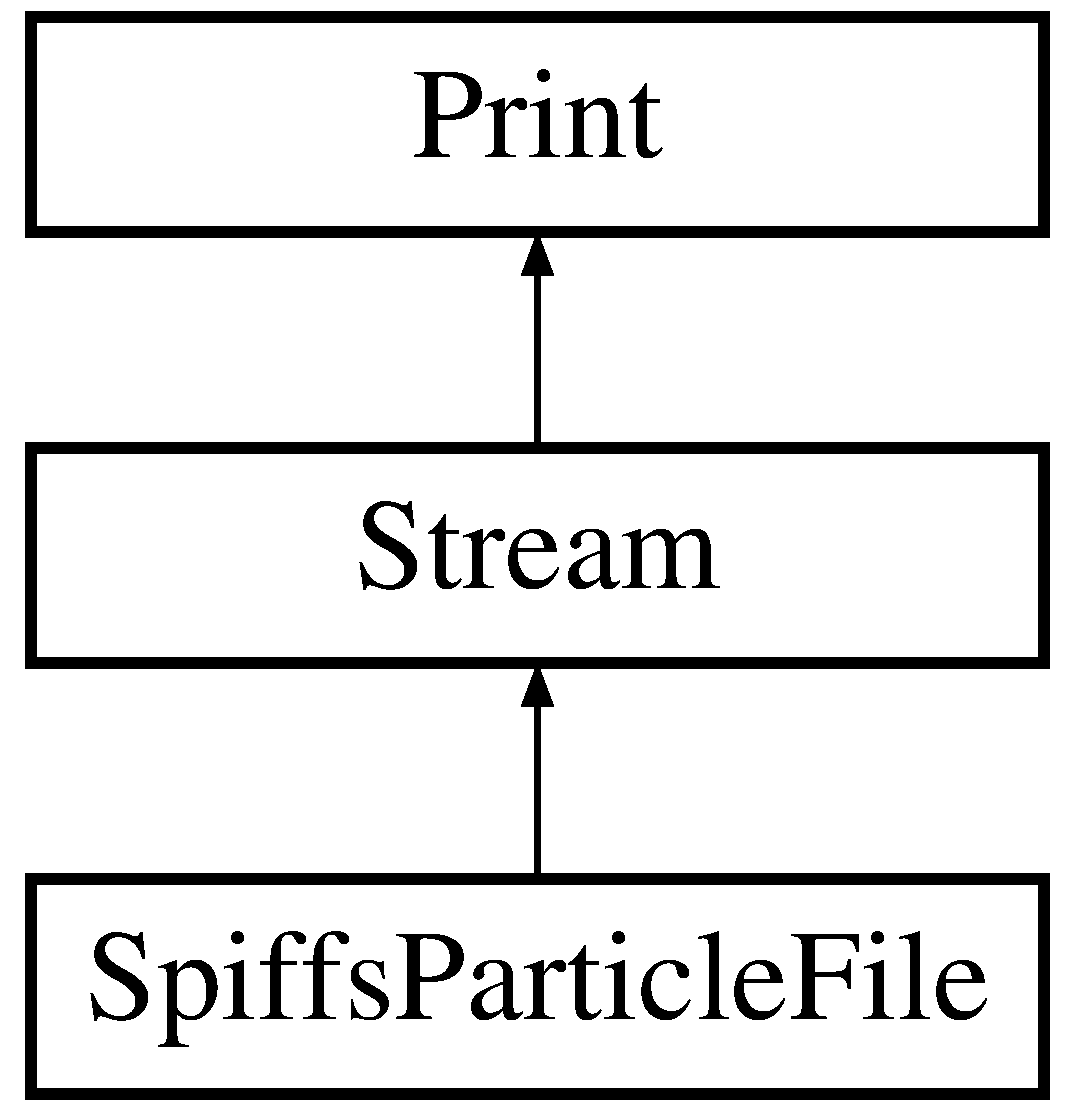
\includegraphics[height=3.000000cm]{class_spiffs_particle_file}
\end{center}
\end{figure}
\subsection*{Public Member Functions}
\begin{DoxyCompactItemize}
\item 
\mbox{\Hypertarget{class_spiffs_particle_file_ae1d791cb24dd193cb76297f37c2902ac}\label{class_spiffs_particle_file_ae1d791cb24dd193cb76297f37c2902ac}} 
\mbox{\hyperlink{class_spiffs_particle_file_ae1d791cb24dd193cb76297f37c2902ac}{Spiffs\+Particle\+File}} ()
\begin{DoxyCompactList}\small\item\em You normally don\textquotesingle{}t need to instantiate one of these, you use the {\ttfamily open\+File} method of \mbox{\hyperlink{class_spiffs_particle}{Spiffs\+Particle}} instead. \end{DoxyCompactList}\item 
\mbox{\Hypertarget{class_spiffs_particle_file_a632c82180b1235744301f5eb88168c5b}\label{class_spiffs_particle_file_a632c82180b1235744301f5eb88168c5b}} 
\mbox{\hyperlink{class_spiffs_particle_file_a632c82180b1235744301f5eb88168c5b}{Spiffs\+Particle\+File}} (\mbox{\hyperlink{structspiffs__t}{spiffs\+\_\+t}} $\ast$fs, spiffs\+\_\+file fh)
\begin{DoxyCompactList}\small\item\em You normally don\textquotesingle{}t need to instantiate one of these, you use the {\ttfamily open\+File} method of \mbox{\hyperlink{class_spiffs_particle}{Spiffs\+Particle}} instead. \end{DoxyCompactList}\item 
\mbox{\Hypertarget{class_spiffs_particle_file_a8d5ba5d2abd9082bc1dab48a2c5aa685}\label{class_spiffs_particle_file_a8d5ba5d2abd9082bc1dab48a2c5aa685}} 
virtual \mbox{\hyperlink{class_spiffs_particle_file_a8d5ba5d2abd9082bc1dab48a2c5aa685}{$\sim$\+Spiffs\+Particle\+File}} ()
\begin{DoxyCompactList}\small\item\em Destructor. Note that this only destroys the container, the underlying file handle is still open and valid. \end{DoxyCompactList}\item 
\mbox{\Hypertarget{class_spiffs_particle_file_ab8d1c9d77137ae02336caad3ee4503af}\label{class_spiffs_particle_file_ab8d1c9d77137ae02336caad3ee4503af}} 
\mbox{\hyperlink{class_spiffs_particle_file_ab8d1c9d77137ae02336caad3ee4503af}{Spiffs\+Particle\+File}} (const \mbox{\hyperlink{class_spiffs_particle_file}{Spiffs\+Particle\+File}} \&other)
\begin{DoxyCompactList}\small\item\em You normally don\textquotesingle{}t need to instantiate one of these, you use the {\ttfamily open\+File} method of \mbox{\hyperlink{class_spiffs_particle}{Spiffs\+Particle}} instead. \end{DoxyCompactList}\item 
\mbox{\hyperlink{class_spiffs_particle_file}{Spiffs\+Particle\+File}} \& \mbox{\hyperlink{class_spiffs_particle_file_aa06d87b0322a764519c5d9726da7b090}{operator=}} (const \mbox{\hyperlink{class_spiffs_particle_file}{Spiffs\+Particle\+File}} \&other)
\begin{DoxyCompactList}\small\item\em You can copy this object, so it\textquotesingle{}s safe to assign it to a local variable. \end{DoxyCompactList}\item 
virtual int \mbox{\hyperlink{class_spiffs_particle_file_a0f1c61016a86835e325bf231d90f9fbf}{available}} ()
\begin{DoxyCompactList}\small\item\em Returns the number of bytes available to read from the current file position. \end{DoxyCompactList}\item 
virtual int \mbox{\hyperlink{class_spiffs_particle_file_a00ff81c014bb8373b3031e4b6ea48c16}{read}} ()
\begin{DoxyCompactList}\small\item\em Read a single byte from the current file position and increment the file position. \end{DoxyCompactList}\item 
virtual int \mbox{\hyperlink{class_spiffs_particle_file_a2d6135f557d39fa6229aea72f8aab855}{peek}} ()
\begin{DoxyCompactList}\small\item\em Read a single byte from the current file position, but do not increment the file position. \end{DoxyCompactList}\item 
virtual void \mbox{\hyperlink{class_spiffs_particle_file_a25a803a411c55fe0ddf1c5d2576d8055}{flush}} ()
\begin{DoxyCompactList}\small\item\em Write any buffered output. \end{DoxyCompactList}\item 
virtual size\+\_\+t \mbox{\hyperlink{class_spiffs_particle_file_a389c6c38e856bb76ac7c0194d7b63ff8}{read\+Bytes}} (char $\ast$buffer, size\+\_\+t \mbox{\hyperlink{class_spiffs_particle_file_ab8b0e24661334106f1eef15bd92bf2e2}{length}})
\begin{DoxyCompactList}\small\item\em Read a specified number of bytes from the file. \end{DoxyCompactList}\item 
virtual size\+\_\+t \mbox{\hyperlink{class_spiffs_particle_file_a073ab7a5701a616959685c58a79e3391}{write}} (uint8\+\_\+t c)
\begin{DoxyCompactList}\small\item\em Write a single byte to the current file position and increment the file position. \end{DoxyCompactList}\item 
virtual size\+\_\+t \mbox{\hyperlink{class_spiffs_particle_file_ada3fa1782a929e32adab1c161f9d5eeb}{write}} (const uint8\+\_\+t $\ast$buffer, size\+\_\+t size)
\begin{DoxyCompactList}\small\item\em Write bytes to the current file position and increment the file position. \end{DoxyCompactList}\item 
s32\+\_\+t \mbox{\hyperlink{class_spiffs_particle_file_a5aeceaf038f055a50376a500dfb27856}{lseek}} (s32\+\_\+t offs, int whence)
\begin{DoxyCompactList}\small\item\em Adjust the file position for reading or writing. \end{DoxyCompactList}\item 
bool \mbox{\hyperlink{class_spiffs_particle_file_adc5b9b4d2447c8a3f1a63b40fd80e56f}{eof}} ()
\begin{DoxyCompactList}\small\item\em Returns true of the file position is currently at the end of the file. \end{DoxyCompactList}\item 
s32\+\_\+t \mbox{\hyperlink{class_spiffs_particle_file_ac1cb4c1027e6e635aff6864efedd0faa}{tell}} ()
\begin{DoxyCompactList}\small\item\em Return the current file position from the start of the file. \end{DoxyCompactList}\item 
s32\+\_\+t \mbox{\hyperlink{class_spiffs_particle_file_ab8b0e24661334106f1eef15bd92bf2e2}{length}} ()
\begin{DoxyCompactList}\small\item\em Returns the length of the file in bytes. \end{DoxyCompactList}\item 
s32\+\_\+t \mbox{\hyperlink{class_spiffs_particle_file_a0a5b83d74718f890d0e449fb7c3bf818}{remove}} ()
\begin{DoxyCompactList}\small\item\em Delete the currently open file. \end{DoxyCompactList}\item 
s32\+\_\+t \mbox{\hyperlink{class_spiffs_particle_file_ae6d57777d56e7594d811c0e7e0e74eab}{truncate}} (s32\+\_\+t len)
\begin{DoxyCompactList}\small\item\em Truncate the currently open file to the specified number of bytes. \end{DoxyCompactList}\item 
\mbox{\Hypertarget{class_spiffs_particle_file_abc5ffc192fa134728111aff8a2105592}\label{class_spiffs_particle_file_abc5ffc192fa134728111aff8a2105592}} 
void \mbox{\hyperlink{class_spiffs_particle_file_abc5ffc192fa134728111aff8a2105592}{seek\+Start}} ()
\begin{DoxyCompactList}\small\item\em Convenience function to move the file position to the beginning of the file. \end{DoxyCompactList}\item 
\mbox{\Hypertarget{class_spiffs_particle_file_a7bb1b4420d8a42cdc66db29d0a5bc1a8}\label{class_spiffs_particle_file_a7bb1b4420d8a42cdc66db29d0a5bc1a8}} 
void \mbox{\hyperlink{class_spiffs_particle_file_a7bb1b4420d8a42cdc66db29d0a5bc1a8}{seek\+End}} ()
\begin{DoxyCompactList}\small\item\em Convenience function to move the file position to the end of the file. \end{DoxyCompactList}\item 
\mbox{\Hypertarget{class_spiffs_particle_file_a0dd9ea24f86d4639ed83e24101968298}\label{class_spiffs_particle_file_a0dd9ea24f86d4639ed83e24101968298}} 
void \mbox{\hyperlink{class_spiffs_particle_file_a0dd9ea24f86d4639ed83e24101968298}{close}} ()
\begin{DoxyCompactList}\small\item\em Close this file. Make sure you close a file when done as there are a finite number of open file available. \end{DoxyCompactList}\item 
bool \mbox{\hyperlink{class_spiffs_particle_file_aa47bab32911760edd8477bcd54f1271d}{is\+Valid}} () const
\begin{DoxyCompactList}\small\item\em Returns true if this object appears to be valid. \end{DoxyCompactList}\item 
\mbox{\Hypertarget{class_spiffs_particle_file_adc7aa6681c2f95cc2d59a54ef7dad2f9}\label{class_spiffs_particle_file_adc7aa6681c2f95cc2d59a54ef7dad2f9}} 
\mbox{\hyperlink{class_spiffs_particle_file_adc7aa6681c2f95cc2d59a54ef7dad2f9}{operator spiffs\+\_\+file}} ()
\begin{DoxyCompactList}\small\item\em Get the underlying S\+P\+I\+F\+FS file handle for this file. \end{DoxyCompactList}\end{DoxyCompactItemize}


\subsection{Detailed Description}
Extension of Arduino/\+Wiring Stream/\+Print manipulating a single S\+P\+I\+F\+FS file. 

Spiffs\+Particle\+RK -\/ Particle wrapper for S\+P\+I\+F\+FS library

Port\+: \href{https://github.com/rickkas7/SpiffsParticleRK}{\tt https\+://github.\+com/rickkas7/\+Spiffs\+Particle\+RK} Original\+: \href{https://github.com/pellepl/spiffs/}{\tt https\+://github.\+com/pellepl/spiffs/}

License\+: M\+IT You can use either this A\+PI, or the native S\+P\+I\+F\+FS A\+PI, which looks basically like the Unix file A\+PI. 

\subsection{Member Function Documentation}
\mbox{\Hypertarget{class_spiffs_particle_file_a0f1c61016a86835e325bf231d90f9fbf}\label{class_spiffs_particle_file_a0f1c61016a86835e325bf231d90f9fbf}} 
\index{Spiffs\+Particle\+File@{Spiffs\+Particle\+File}!available@{available}}
\index{available@{available}!Spiffs\+Particle\+File@{Spiffs\+Particle\+File}}
\subsubsection{\texorpdfstring{available()}{available()}}
{\footnotesize\ttfamily int Spiffs\+Particle\+File\+::available (\begin{DoxyParamCaption}{ }\end{DoxyParamCaption})\hspace{0.3cm}{\ttfamily [virtual]}}



Returns the number of bytes available to read from the current file position. 

This is a standard Arduino/\+Wiring method for \mbox{\hyperlink{class_stream}{Stream}} objects. 

Implements \mbox{\hyperlink{class_stream_a9c98a763395005c08ce95afb2f06c7b1}{Stream}}.

\mbox{\Hypertarget{class_spiffs_particle_file_adc5b9b4d2447c8a3f1a63b40fd80e56f}\label{class_spiffs_particle_file_adc5b9b4d2447c8a3f1a63b40fd80e56f}} 
\index{Spiffs\+Particle\+File@{Spiffs\+Particle\+File}!eof@{eof}}
\index{eof@{eof}!Spiffs\+Particle\+File@{Spiffs\+Particle\+File}}
\subsubsection{\texorpdfstring{eof()}{eof()}}
{\footnotesize\ttfamily bool Spiffs\+Particle\+File\+::eof (\begin{DoxyParamCaption}{ }\end{DoxyParamCaption})\hspace{0.3cm}{\ttfamily [inline]}}



Returns true of the file position is currently at the end of the file. 

\begin{DoxyReturn}{Returns}
true if at end of file, false if not 
\end{DoxyReturn}
\mbox{\Hypertarget{class_spiffs_particle_file_a25a803a411c55fe0ddf1c5d2576d8055}\label{class_spiffs_particle_file_a25a803a411c55fe0ddf1c5d2576d8055}} 
\index{Spiffs\+Particle\+File@{Spiffs\+Particle\+File}!flush@{flush}}
\index{flush@{flush}!Spiffs\+Particle\+File@{Spiffs\+Particle\+File}}
\subsubsection{\texorpdfstring{flush()}{flush()}}
{\footnotesize\ttfamily void Spiffs\+Particle\+File\+::flush (\begin{DoxyParamCaption}{ }\end{DoxyParamCaption})\hspace{0.3cm}{\ttfamily [virtual]}}



Write any buffered output. 

It is not necessary to flush before close, as close will automatically flush any output if necessary.

This is a standard Arduino/\+Wiring method for \mbox{\hyperlink{class_stream}{Stream}} objects. 

Implements \mbox{\hyperlink{class_stream_aa3ef2c34f152a0b2ea8de9139b9461da}{Stream}}.

\mbox{\Hypertarget{class_spiffs_particle_file_aa47bab32911760edd8477bcd54f1271d}\label{class_spiffs_particle_file_aa47bab32911760edd8477bcd54f1271d}} 
\index{Spiffs\+Particle\+File@{Spiffs\+Particle\+File}!is\+Valid@{is\+Valid}}
\index{is\+Valid@{is\+Valid}!Spiffs\+Particle\+File@{Spiffs\+Particle\+File}}
\subsubsection{\texorpdfstring{is\+Valid()}{isValid()}}
{\footnotesize\ttfamily bool Spiffs\+Particle\+File\+::is\+Valid (\begin{DoxyParamCaption}{ }\end{DoxyParamCaption}) const\hspace{0.3cm}{\ttfamily [inline]}}



Returns true if this object appears to be valid. 

This is mainly used when using the open\+File method. Since this object is returned, you use the \mbox{\hyperlink{class_spiffs_particle_file_aa47bab32911760edd8477bcd54f1271d}{is\+Valid()}} method to find out if the open\+File succeeded. It might not if you try to open without create a file that does not exist, for example. \mbox{\Hypertarget{class_spiffs_particle_file_ab8b0e24661334106f1eef15bd92bf2e2}\label{class_spiffs_particle_file_ab8b0e24661334106f1eef15bd92bf2e2}} 
\index{Spiffs\+Particle\+File@{Spiffs\+Particle\+File}!length@{length}}
\index{length@{length}!Spiffs\+Particle\+File@{Spiffs\+Particle\+File}}
\subsubsection{\texorpdfstring{length()}{length()}}
{\footnotesize\ttfamily s32\+\_\+t Spiffs\+Particle\+File\+::length (\begin{DoxyParamCaption}{ }\end{DoxyParamCaption})}



Returns the length of the file in bytes. 

\begin{DoxyReturn}{Returns}
the length of the file in bytes or a negative error code 
\end{DoxyReturn}
\mbox{\Hypertarget{class_spiffs_particle_file_a5aeceaf038f055a50376a500dfb27856}\label{class_spiffs_particle_file_a5aeceaf038f055a50376a500dfb27856}} 
\index{Spiffs\+Particle\+File@{Spiffs\+Particle\+File}!lseek@{lseek}}
\index{lseek@{lseek}!Spiffs\+Particle\+File@{Spiffs\+Particle\+File}}
\subsubsection{\texorpdfstring{lseek()}{lseek()}}
{\footnotesize\ttfamily s32\+\_\+t Spiffs\+Particle\+File\+::lseek (\begin{DoxyParamCaption}\item[{s32\+\_\+t}]{offs,  }\item[{int}]{whence }\end{DoxyParamCaption})\hspace{0.3cm}{\ttfamily [inline]}}



Adjust the file position for reading or writing. 


\begin{DoxyParams}{Parameters}
{\em offs} & Offset, can be positive or negative\\
\hline
{\em whence} & Offset relative to what\+:\\
\hline
\end{DoxyParams}

\begin{DoxyItemize}
\item S\+P\+I\+F\+F\+S\+\_\+\+S\+E\+E\+K\+\_\+\+S\+ET the beginning of the file
\item S\+P\+I\+F\+F\+S\+\_\+\+S\+E\+E\+K\+\_\+\+C\+UR the current file position
\item S\+P\+I\+F\+F\+S\+\_\+\+S\+E\+E\+K\+\_\+\+E\+ND the end of the file
\end{DoxyItemize}

\begin{DoxyReturn}{Returns}
S\+P\+I\+F\+F\+S\+\_\+\+OK (0) on success, or a negative S\+P\+I\+F\+F\+S\+\_\+\+E\+RR code.
\end{DoxyReturn}
This is a wrapper for the S\+P\+I\+F\+FS call, which emulates the Unix/\+P\+O\+S\+IX A\+PI. \mbox{\Hypertarget{class_spiffs_particle_file_aa06d87b0322a764519c5d9726da7b090}\label{class_spiffs_particle_file_aa06d87b0322a764519c5d9726da7b090}} 
\index{Spiffs\+Particle\+File@{Spiffs\+Particle\+File}!operator=@{operator=}}
\index{operator=@{operator=}!Spiffs\+Particle\+File@{Spiffs\+Particle\+File}}
\subsubsection{\texorpdfstring{operator=()}{operator=()}}
{\footnotesize\ttfamily \mbox{\hyperlink{class_spiffs_particle_file}{Spiffs\+Particle\+File}} \& Spiffs\+Particle\+File\+::operator= (\begin{DoxyParamCaption}\item[{const \mbox{\hyperlink{class_spiffs_particle_file}{Spiffs\+Particle\+File}} \&}]{other }\end{DoxyParamCaption})}



You can copy this object, so it\textquotesingle{}s safe to assign it to a local variable. 

This object is only a container for the file handle; it doesn\textquotesingle{}t do any reference counting and the file handle is only closed if you call the \mbox{\hyperlink{class_spiffs_particle_file_a0dd9ea24f86d4639ed83e24101968298}{close()}} method; deleting this object or letting it go out of scope doesn\textquotesingle{}t close the file handle. \mbox{\Hypertarget{class_spiffs_particle_file_a2d6135f557d39fa6229aea72f8aab855}\label{class_spiffs_particle_file_a2d6135f557d39fa6229aea72f8aab855}} 
\index{Spiffs\+Particle\+File@{Spiffs\+Particle\+File}!peek@{peek}}
\index{peek@{peek}!Spiffs\+Particle\+File@{Spiffs\+Particle\+File}}
\subsubsection{\texorpdfstring{peek()}{peek()}}
{\footnotesize\ttfamily int Spiffs\+Particle\+File\+::peek (\begin{DoxyParamCaption}{ }\end{DoxyParamCaption})\hspace{0.3cm}{\ttfamily [virtual]}}



Read a single byte from the current file position, but do not increment the file position. 

\begin{DoxyReturn}{Returns}
a byte value 0 -\/ 255 or -\/1 if at the end of file.
\end{DoxyReturn}
This is a standard Arduino/\+Wiring method for \mbox{\hyperlink{class_stream}{Stream}} objects. 

Implements \mbox{\hyperlink{class_stream_a30c3c212ec6ea67277a708c5ea2501a5}{Stream}}.

\mbox{\Hypertarget{class_spiffs_particle_file_a00ff81c014bb8373b3031e4b6ea48c16}\label{class_spiffs_particle_file_a00ff81c014bb8373b3031e4b6ea48c16}} 
\index{Spiffs\+Particle\+File@{Spiffs\+Particle\+File}!read@{read}}
\index{read@{read}!Spiffs\+Particle\+File@{Spiffs\+Particle\+File}}
\subsubsection{\texorpdfstring{read()}{read()}}
{\footnotesize\ttfamily int Spiffs\+Particle\+File\+::read (\begin{DoxyParamCaption}{ }\end{DoxyParamCaption})\hspace{0.3cm}{\ttfamily [virtual]}}



Read a single byte from the current file position and increment the file position. 

\begin{DoxyReturn}{Returns}
a byte value 0 -\/ 255 or -\/1 if at the end of file.
\end{DoxyReturn}
This is a standard Arduino/\+Wiring method for \mbox{\hyperlink{class_stream}{Stream}} objects. 

Implements \mbox{\hyperlink{class_stream_aea5dee9fcb038148515b7c9212d38dc0}{Stream}}.

\mbox{\Hypertarget{class_spiffs_particle_file_a389c6c38e856bb76ac7c0194d7b63ff8}\label{class_spiffs_particle_file_a389c6c38e856bb76ac7c0194d7b63ff8}} 
\index{Spiffs\+Particle\+File@{Spiffs\+Particle\+File}!read\+Bytes@{read\+Bytes}}
\index{read\+Bytes@{read\+Bytes}!Spiffs\+Particle\+File@{Spiffs\+Particle\+File}}
\subsubsection{\texorpdfstring{read\+Bytes()}{readBytes()}}
{\footnotesize\ttfamily size\+\_\+t Spiffs\+Particle\+File\+::read\+Bytes (\begin{DoxyParamCaption}\item[{char $\ast$}]{buffer,  }\item[{size\+\_\+t}]{length }\end{DoxyParamCaption})\hspace{0.3cm}{\ttfamily [virtual]}}



Read a specified number of bytes from the file. 


\begin{DoxyParams}{Parameters}
{\em buffer} & The buffer to write to\\
\hline
{\em length} & The number of bytes to read. It may read less than that.\\
\hline
\end{DoxyParams}
\begin{DoxyReturn}{Returns}
The number of bytes read, which will be 0 to length bytes.
\end{DoxyReturn}
This is a standard Arduino/\+Wiring method for \mbox{\hyperlink{class_stream}{Stream}} objects. \mbox{\Hypertarget{class_spiffs_particle_file_a0a5b83d74718f890d0e449fb7c3bf818}\label{class_spiffs_particle_file_a0a5b83d74718f890d0e449fb7c3bf818}} 
\index{Spiffs\+Particle\+File@{Spiffs\+Particle\+File}!remove@{remove}}
\index{remove@{remove}!Spiffs\+Particle\+File@{Spiffs\+Particle\+File}}
\subsubsection{\texorpdfstring{remove()}{remove()}}
{\footnotesize\ttfamily s32\+\_\+t Spiffs\+Particle\+File\+::remove (\begin{DoxyParamCaption}{ }\end{DoxyParamCaption})\hspace{0.3cm}{\ttfamily [inline]}}



Delete the currently open file. 

Note that the \mbox{\hyperlink{class_spiffs_particle}{Spiffs\+Particle}} class has a method to delete a file by filename, this method is provided if you already have the file open.

\begin{DoxyReturn}{Returns}
S\+P\+I\+F\+F\+S\+\_\+\+OK (0) on success, or a negative S\+P\+I\+F\+F\+S\+\_\+\+E\+RR code. 
\end{DoxyReturn}
\mbox{\Hypertarget{class_spiffs_particle_file_ac1cb4c1027e6e635aff6864efedd0faa}\label{class_spiffs_particle_file_ac1cb4c1027e6e635aff6864efedd0faa}} 
\index{Spiffs\+Particle\+File@{Spiffs\+Particle\+File}!tell@{tell}}
\index{tell@{tell}!Spiffs\+Particle\+File@{Spiffs\+Particle\+File}}
\subsubsection{\texorpdfstring{tell()}{tell()}}
{\footnotesize\ttfamily s32\+\_\+t Spiffs\+Particle\+File\+::tell (\begin{DoxyParamCaption}{ }\end{DoxyParamCaption})\hspace{0.3cm}{\ttfamily [inline]}}



Return the current file position from the start of the file. 

\begin{DoxyReturn}{Returns}
file position (0 = at the start of the file) or a negative error code
\end{DoxyReturn}
This is a wrapper for the S\+P\+I\+F\+FS call, which emulates the Unix/\+P\+O\+S\+IX A\+PI. \mbox{\Hypertarget{class_spiffs_particle_file_ae6d57777d56e7594d811c0e7e0e74eab}\label{class_spiffs_particle_file_ae6d57777d56e7594d811c0e7e0e74eab}} 
\index{Spiffs\+Particle\+File@{Spiffs\+Particle\+File}!truncate@{truncate}}
\index{truncate@{truncate}!Spiffs\+Particle\+File@{Spiffs\+Particle\+File}}
\subsubsection{\texorpdfstring{truncate()}{truncate()}}
{\footnotesize\ttfamily s32\+\_\+t Spiffs\+Particle\+File\+::truncate (\begin{DoxyParamCaption}\item[{s32\+\_\+t}]{len }\end{DoxyParamCaption})\hspace{0.3cm}{\ttfamily [inline]}}



Truncate the currently open file to the specified number of bytes. 

Note that in P\+O\+S\+IX, you can truncate a file to make it longer than the current file length but in S\+P\+I\+F\+FS you can only truncate a file to be equal to or less than the current file length.

\begin{DoxyReturn}{Returns}
S\+P\+I\+F\+F\+S\+\_\+\+OK (0) on success, or a negative S\+P\+I\+F\+F\+S\+\_\+\+E\+RR code. 
\end{DoxyReturn}
\mbox{\Hypertarget{class_spiffs_particle_file_a073ab7a5701a616959685c58a79e3391}\label{class_spiffs_particle_file_a073ab7a5701a616959685c58a79e3391}} 
\index{Spiffs\+Particle\+File@{Spiffs\+Particle\+File}!write@{write}}
\index{write@{write}!Spiffs\+Particle\+File@{Spiffs\+Particle\+File}}
\subsubsection{\texorpdfstring{write()}{write()}\hspace{0.1cm}{\footnotesize\ttfamily [1/2]}}
{\footnotesize\ttfamily size\+\_\+t Spiffs\+Particle\+File\+::write (\begin{DoxyParamCaption}\item[{uint8\+\_\+t}]{c }\end{DoxyParamCaption})\hspace{0.3cm}{\ttfamily [virtual]}}



Write a single byte to the current file position and increment the file position. 


\begin{DoxyParams}{Parameters}
{\em c} & The byte to write. Can write binary or text data.\\
\hline
\end{DoxyParams}
This is a standard Arduino/\+Wiring method for \mbox{\hyperlink{class_stream}{Stream}} objects. 

Implements \mbox{\hyperlink{class_print_a5be30d49adae2406a270c29ba9a3e0a3}{Print}}.

\mbox{\Hypertarget{class_spiffs_particle_file_ada3fa1782a929e32adab1c161f9d5eeb}\label{class_spiffs_particle_file_ada3fa1782a929e32adab1c161f9d5eeb}} 
\index{Spiffs\+Particle\+File@{Spiffs\+Particle\+File}!write@{write}}
\index{write@{write}!Spiffs\+Particle\+File@{Spiffs\+Particle\+File}}
\subsubsection{\texorpdfstring{write()}{write()}\hspace{0.1cm}{\footnotesize\ttfamily [2/2]}}
{\footnotesize\ttfamily size\+\_\+t Spiffs\+Particle\+File\+::write (\begin{DoxyParamCaption}\item[{const uint8\+\_\+t $\ast$}]{buffer,  }\item[{size\+\_\+t}]{size }\end{DoxyParamCaption})\hspace{0.3cm}{\ttfamily [virtual]}}



Write bytes to the current file position and increment the file position. 


\begin{DoxyParams}{Parameters}
{\em buffer} & The buffer to write. Can write binary or text data.\\
\hline
{\em length} & The number of bytes to write.\\
\hline
\end{DoxyParams}
\begin{DoxyReturn}{Returns}
The number of bytes written, typically this will be length.
\end{DoxyReturn}
This is a standard Arduino/\+Wiring method for \mbox{\hyperlink{class_stream}{Stream}} objects. 

Reimplemented from \mbox{\hyperlink{class_print_a88864e109589a5be9b0f5ba1327f8421}{Print}}.



The documentation for this class was generated from the following files\+:\begin{DoxyCompactItemize}
\item 
src/Spiffs\+Particle\+R\+K.\+h\item 
src/Spiffs\+Particle\+R\+K.\+cpp\end{DoxyCompactItemize}

\hypertarget{class_stream}{}\section{Stream Class Reference}
\label{class_stream}\index{Stream@{Stream}}


Arduino/\+Wiring \mbox{\hyperlink{class_stream}{Stream}} Class.  




{\ttfamily \#include $<$spark\+\_\+wiring\+\_\+stream.\+h$>$}

Inheritance diagram for Stream\+:\begin{figure}[H]
\begin{center}
\leavevmode
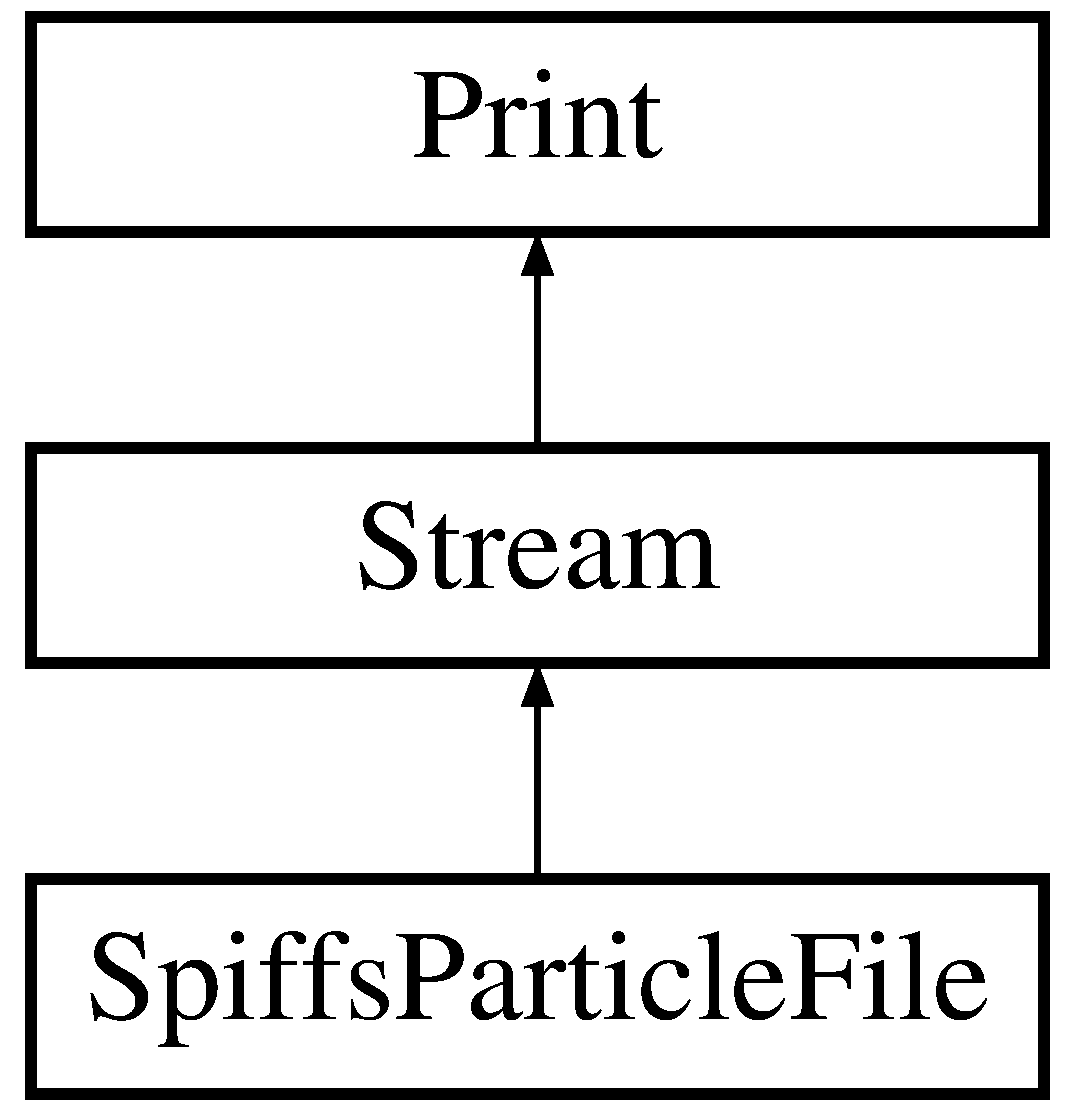
\includegraphics[height=3.000000cm]{class_stream}
\end{center}
\end{figure}
\subsection*{Public Member Functions}
\begin{DoxyCompactItemize}
\item 
virtual int \mbox{\hyperlink{class_stream_a9c98a763395005c08ce95afb2f06c7b1}{available}} ()=0
\begin{DoxyCompactList}\small\item\em Returns the number of a bytes available to read right now. \end{DoxyCompactList}\item 
virtual int \mbox{\hyperlink{class_stream_aea5dee9fcb038148515b7c9212d38dc0}{read}} ()=0
\begin{DoxyCompactList}\small\item\em Read a byte from the stream. \end{DoxyCompactList}\item 
virtual int \mbox{\hyperlink{class_stream_a30c3c212ec6ea67277a708c5ea2501a5}{peek}} ()=0
\begin{DoxyCompactList}\small\item\em Read a byte from the stream but do not remove it so read will return the same byte next time. \end{DoxyCompactList}\item 
\mbox{\Hypertarget{class_stream_aa3ef2c34f152a0b2ea8de9139b9461da}\label{class_stream_aa3ef2c34f152a0b2ea8de9139b9461da}} 
virtual void \mbox{\hyperlink{class_stream_aa3ef2c34f152a0b2ea8de9139b9461da}{flush}} ()=0
\begin{DoxyCompactList}\small\item\em For output streams, writes any unwritten buffered data. \end{DoxyCompactList}\item 
void \mbox{\hyperlink{class_stream_abaa50647d6dbb3baf7697a2691a06177}{set\+Timeout}} (system\+\_\+tick\+\_\+t timeout)
\begin{DoxyCompactList}\small\item\em Sets the read timeout (default\+: 1000 milliseconds) \end{DoxyCompactList}\item 
bool \mbox{\hyperlink{class_stream_a4bab30ccd324efd461dee46a2339f673}{find}} (char $\ast$target)
\begin{DoxyCompactList}\small\item\em Reads data from the stream until the target string is found. \end{DoxyCompactList}\item 
bool \mbox{\hyperlink{class_stream_ad851401f2318cdb1de05707e021b81d9}{find}} (char $\ast$target, size\+\_\+t length)
\begin{DoxyCompactList}\small\item\em Reads data from the stream until the target string is found. \end{DoxyCompactList}\item 
bool \mbox{\hyperlink{class_stream_ad1f5f6600832396fb38a897baf4de35b}{find\+Until}} (char $\ast$target, char $\ast$terminator)
\begin{DoxyCompactList}\small\item\em Reads data from the stream until the target string is found or the terminator string is found. \end{DoxyCompactList}\item 
bool \mbox{\hyperlink{class_stream_a3a9497de614792103ab8cb4759e01a69}{find\+Until}} (char $\ast$target, size\+\_\+t target\+Len, char $\ast$terminate, size\+\_\+t term\+Len)
\begin{DoxyCompactList}\small\item\em Reads data from the stream until the target string is found or the terminator string is found. \end{DoxyCompactList}\item 
long \mbox{\hyperlink{class_stream_a497ffcbcb4d5bb889a8fde487bcc1b98}{parse\+Int}} ()
\begin{DoxyCompactList}\small\item\em returns the first valid (long) integer value from the current position \end{DoxyCompactList}\item 
float \mbox{\hyperlink{class_stream_a5e5a0cc11eb586d89dcb7fa8e53a87e8}{parse\+Float}} ()
\begin{DoxyCompactList}\small\item\em returns the first valid float value from the current position \end{DoxyCompactList}\item 
size\+\_\+t \mbox{\hyperlink{class_stream_a45fd1336a323ea83b16e8507055f44ea}{read\+Bytes}} (char $\ast$buffer, size\+\_\+t length)
\begin{DoxyCompactList}\small\item\em Read chars from stream into buffer. \end{DoxyCompactList}\item 
size\+\_\+t \mbox{\hyperlink{class_stream_af84672a4fb2620466958d3118d4fea00}{read\+Bytes\+Until}} (char terminator, char $\ast$buffer, size\+\_\+t length)
\begin{DoxyCompactList}\small\item\em Read chars from stream into buffer until the character terminator is found. \end{DoxyCompactList}\item 
\mbox{\Hypertarget{class_stream_a1c60bdda2b65d78e5a1362d51b856c5a}\label{class_stream_a1c60bdda2b65d78e5a1362d51b856c5a}} 
String \mbox{\hyperlink{class_stream_a1c60bdda2b65d78e5a1362d51b856c5a}{read\+String}} ()
\begin{DoxyCompactList}\small\item\em Reads the remainder of the file into a string. \end{DoxyCompactList}\item 
String \mbox{\hyperlink{class_stream_a6a409da87c552909260d8cc428c5ca70}{read\+String\+Until}} (char terminator)
\begin{DoxyCompactList}\small\item\em Reads the remainder of the file into a string or until terminator is found. \end{DoxyCompactList}\end{DoxyCompactItemize}


\subsection{Detailed Description}
Arduino/\+Wiring \mbox{\hyperlink{class_stream}{Stream}} Class. 

Methods for reading data from a stream, such a serial port, T\+CP network stream, or a file. 

\subsection{Member Function Documentation}
\mbox{\Hypertarget{class_stream_a9c98a763395005c08ce95afb2f06c7b1}\label{class_stream_a9c98a763395005c08ce95afb2f06c7b1}} 
\index{Stream@{Stream}!available@{available}}
\index{available@{available}!Stream@{Stream}}
\subsubsection{\texorpdfstring{available()}{available()}}
{\footnotesize\ttfamily virtual int Stream\+::available (\begin{DoxyParamCaption}{ }\end{DoxyParamCaption})\hspace{0.3cm}{\ttfamily [pure virtual]}}



Returns the number of a bytes available to read right now. 

For files, the number of bytes left to read in the file from the current file position. 

Implemented in \mbox{\hyperlink{class_spiffs_particle_file_a0f1c61016a86835e325bf231d90f9fbf}{Spiffs\+Particle\+File}}.

\mbox{\Hypertarget{class_stream_a4bab30ccd324efd461dee46a2339f673}\label{class_stream_a4bab30ccd324efd461dee46a2339f673}} 
\index{Stream@{Stream}!find@{find}}
\index{find@{find}!Stream@{Stream}}
\subsubsection{\texorpdfstring{find()}{find()}\hspace{0.1cm}{\footnotesize\ttfamily [1/2]}}
{\footnotesize\ttfamily bool Stream\+::find (\begin{DoxyParamCaption}\item[{char $\ast$}]{target }\end{DoxyParamCaption})}



Reads data from the stream until the target string is found. 


\begin{DoxyParams}{Parameters}
{\em target} & The string to search for (null-\/terminated c-\/string)\\
\hline
\end{DoxyParams}
\begin{DoxyReturn}{Returns}
true if target string is found, false if timed out (see set\+Timeout) 
\end{DoxyReturn}
\mbox{\Hypertarget{class_stream_ad851401f2318cdb1de05707e021b81d9}\label{class_stream_ad851401f2318cdb1de05707e021b81d9}} 
\index{Stream@{Stream}!find@{find}}
\index{find@{find}!Stream@{Stream}}
\subsubsection{\texorpdfstring{find()}{find()}\hspace{0.1cm}{\footnotesize\ttfamily [2/2]}}
{\footnotesize\ttfamily bool Stream\+::find (\begin{DoxyParamCaption}\item[{char $\ast$}]{target,  }\item[{size\+\_\+t}]{length }\end{DoxyParamCaption})}



Reads data from the stream until the target string is found. 


\begin{DoxyParams}{Parameters}
{\em target} & The string to search for. The string is specified by length so it does not need to be null-\/terminated.\\
\hline
{\em length} & The number of bytes in target to search for.\\
\hline
\end{DoxyParams}
\begin{DoxyReturn}{Returns}
true if target string is found, false if timed out (see set\+Timeout) 
\end{DoxyReturn}
\mbox{\Hypertarget{class_stream_ad1f5f6600832396fb38a897baf4de35b}\label{class_stream_ad1f5f6600832396fb38a897baf4de35b}} 
\index{Stream@{Stream}!find\+Until@{find\+Until}}
\index{find\+Until@{find\+Until}!Stream@{Stream}}
\subsubsection{\texorpdfstring{find\+Until()}{findUntil()}\hspace{0.1cm}{\footnotesize\ttfamily [1/2]}}
{\footnotesize\ttfamily bool Stream\+::find\+Until (\begin{DoxyParamCaption}\item[{char $\ast$}]{target,  }\item[{char $\ast$}]{terminator }\end{DoxyParamCaption})}



Reads data from the stream until the target string is found or the terminator string is found. 


\begin{DoxyParams}{Parameters}
{\em target} & The string to search for (null-\/terminated c-\/string)\\
\hline
{\em terminator} & The terminator string to search for (null-\/terminated c-\/string)\\
\hline
\end{DoxyParams}
\begin{DoxyReturn}{Returns}
true if target string is found, false if timed out (see set\+Timeout) 
\end{DoxyReturn}
\mbox{\Hypertarget{class_stream_a3a9497de614792103ab8cb4759e01a69}\label{class_stream_a3a9497de614792103ab8cb4759e01a69}} 
\index{Stream@{Stream}!find\+Until@{find\+Until}}
\index{find\+Until@{find\+Until}!Stream@{Stream}}
\subsubsection{\texorpdfstring{find\+Until()}{findUntil()}\hspace{0.1cm}{\footnotesize\ttfamily [2/2]}}
{\footnotesize\ttfamily bool Stream\+::find\+Until (\begin{DoxyParamCaption}\item[{char $\ast$}]{target,  }\item[{size\+\_\+t}]{target\+Len,  }\item[{char $\ast$}]{terminate,  }\item[{size\+\_\+t}]{term\+Len }\end{DoxyParamCaption})}



Reads data from the stream until the target string is found or the terminator string is found. 


\begin{DoxyParams}{Parameters}
{\em target} & The string to search for. The string is specified by length so it does not need to be null-\/terminated.\\
\hline
{\em length} & The number of bytes in target to search for.\\
\hline
{\em terminator} & The terminator string to search for. The string is specified by length so it does not need to be null-\/terminated.\\
\hline
{\em term\+Len} & The number of bytes in terminator to search for.\\
\hline
\end{DoxyParams}
\begin{DoxyReturn}{Returns}
true if target string is found, false if timed out (see set\+Timeout) 
\end{DoxyReturn}
\mbox{\Hypertarget{class_stream_a5e5a0cc11eb586d89dcb7fa8e53a87e8}\label{class_stream_a5e5a0cc11eb586d89dcb7fa8e53a87e8}} 
\index{Stream@{Stream}!parse\+Float@{parse\+Float}}
\index{parse\+Float@{parse\+Float}!Stream@{Stream}}
\subsubsection{\texorpdfstring{parse\+Float()}{parseFloat()}}
{\footnotesize\ttfamily float Stream\+::parse\+Float (\begin{DoxyParamCaption}{ }\end{DoxyParamCaption})}



returns the first valid float value from the current position 

Initial characters that are not digits (or the minus sign or .) are skipped float is terminated by the first character that is not a float character. Decimal part is separate by \textquotesingle{}.\textquotesingle{}. \mbox{\Hypertarget{class_stream_a497ffcbcb4d5bb889a8fde487bcc1b98}\label{class_stream_a497ffcbcb4d5bb889a8fde487bcc1b98}} 
\index{Stream@{Stream}!parse\+Int@{parse\+Int}}
\index{parse\+Int@{parse\+Int}!Stream@{Stream}}
\subsubsection{\texorpdfstring{parse\+Int()}{parseInt()}}
{\footnotesize\ttfamily long Stream\+::parse\+Int (\begin{DoxyParamCaption}{ }\end{DoxyParamCaption})}



returns the first valid (long) integer value from the current position 

Initial characters that are not digits (or the minus sign) are skipped integer is terminated by the first character that is not a digit. \mbox{\Hypertarget{class_stream_a30c3c212ec6ea67277a708c5ea2501a5}\label{class_stream_a30c3c212ec6ea67277a708c5ea2501a5}} 
\index{Stream@{Stream}!peek@{peek}}
\index{peek@{peek}!Stream@{Stream}}
\subsubsection{\texorpdfstring{peek()}{peek()}}
{\footnotesize\ttfamily virtual int Stream\+::peek (\begin{DoxyParamCaption}{ }\end{DoxyParamCaption})\hspace{0.3cm}{\ttfamily [pure virtual]}}



Read a byte from the stream but do not remove it so read will return the same byte next time. 

\begin{DoxyReturn}{Returns}
A byte value 0 -\/ 255, or -\/1 if there are no bytes available.
\end{DoxyReturn}
For files, the current file position is left unchanged. 

Implemented in \mbox{\hyperlink{class_spiffs_particle_file_a2d6135f557d39fa6229aea72f8aab855}{Spiffs\+Particle\+File}}.

\mbox{\Hypertarget{class_stream_aea5dee9fcb038148515b7c9212d38dc0}\label{class_stream_aea5dee9fcb038148515b7c9212d38dc0}} 
\index{Stream@{Stream}!read@{read}}
\index{read@{read}!Stream@{Stream}}
\subsubsection{\texorpdfstring{read()}{read()}}
{\footnotesize\ttfamily virtual int Stream\+::read (\begin{DoxyParamCaption}{ }\end{DoxyParamCaption})\hspace{0.3cm}{\ttfamily [pure virtual]}}



Read a byte from the stream. 

\begin{DoxyReturn}{Returns}
A byte value 0 -\/ 255, or -\/1 if there are no bytes available. 
\end{DoxyReturn}


Implemented in \mbox{\hyperlink{class_spiffs_particle_file_a00ff81c014bb8373b3031e4b6ea48c16}{Spiffs\+Particle\+File}}.

\mbox{\Hypertarget{class_stream_a45fd1336a323ea83b16e8507055f44ea}\label{class_stream_a45fd1336a323ea83b16e8507055f44ea}} 
\index{Stream@{Stream}!read\+Bytes@{read\+Bytes}}
\index{read\+Bytes@{read\+Bytes}!Stream@{Stream}}
\subsubsection{\texorpdfstring{read\+Bytes()}{readBytes()}}
{\footnotesize\ttfamily size\+\_\+t Stream\+::read\+Bytes (\begin{DoxyParamCaption}\item[{char $\ast$}]{buffer,  }\item[{size\+\_\+t}]{length }\end{DoxyParamCaption})}



Read chars from stream into buffer. 


\begin{DoxyParams}{Parameters}
{\em buffer} & The buffer to read into \\
\hline
{\em length} & The number of bytes to read \\
\hline
\end{DoxyParams}
\begin{DoxyReturn}{Returns}
the number of characters placed in the buffer (0 means no valid data found) 
\end{DoxyReturn}
\mbox{\Hypertarget{class_stream_af84672a4fb2620466958d3118d4fea00}\label{class_stream_af84672a4fb2620466958d3118d4fea00}} 
\index{Stream@{Stream}!read\+Bytes\+Until@{read\+Bytes\+Until}}
\index{read\+Bytes\+Until@{read\+Bytes\+Until}!Stream@{Stream}}
\subsubsection{\texorpdfstring{read\+Bytes\+Until()}{readBytesUntil()}}
{\footnotesize\ttfamily size\+\_\+t Stream\+::read\+Bytes\+Until (\begin{DoxyParamCaption}\item[{char}]{terminator,  }\item[{char $\ast$}]{buffer,  }\item[{size\+\_\+t}]{length }\end{DoxyParamCaption})}



Read chars from stream into buffer until the character terminator is found. 


\begin{DoxyParams}{Parameters}
{\em terminator} & The character to stop reading \\
\hline
{\em buffer} & The buffer to read into \\
\hline
{\em length} & The number of bytes to read \\
\hline
\end{DoxyParams}
\begin{DoxyReturn}{Returns}
the number of characters placed in the buffer (0 means no valid data found)
\end{DoxyReturn}
The terminator could be some thing like \textbackslash{}n (newline), \textbackslash{}t (tab), etc. depending on the data you are parsing. \mbox{\Hypertarget{class_stream_a6a409da87c552909260d8cc428c5ca70}\label{class_stream_a6a409da87c552909260d8cc428c5ca70}} 
\index{Stream@{Stream}!read\+String\+Until@{read\+String\+Until}}
\index{read\+String\+Until@{read\+String\+Until}!Stream@{Stream}}
\subsubsection{\texorpdfstring{read\+String\+Until()}{readStringUntil()}}
{\footnotesize\ttfamily String Stream\+::read\+String\+Until (\begin{DoxyParamCaption}\item[{char}]{terminator }\end{DoxyParamCaption})}



Reads the remainder of the file into a string or until terminator is found. 


\begin{DoxyParams}{Parameters}
{\em terminator} & The character to stop reading \\
\hline
\end{DoxyParams}
\mbox{\Hypertarget{class_stream_abaa50647d6dbb3baf7697a2691a06177}\label{class_stream_abaa50647d6dbb3baf7697a2691a06177}} 
\index{Stream@{Stream}!set\+Timeout@{set\+Timeout}}
\index{set\+Timeout@{set\+Timeout}!Stream@{Stream}}
\subsubsection{\texorpdfstring{set\+Timeout()}{setTimeout()}}
{\footnotesize\ttfamily void Stream\+::set\+Timeout (\begin{DoxyParamCaption}\item[{system\+\_\+tick\+\_\+t}]{timeout }\end{DoxyParamCaption})}



Sets the read timeout (default\+: 1000 milliseconds) 

This makes more sense for network and serial streams. 

The documentation for this class was generated from the following file\+:\begin{DoxyCompactItemize}
\item 
docs/src/\mbox{\hyperlink{spark__wiring__stream_8h}{spark\+\_\+wiring\+\_\+stream.\+h}}\end{DoxyCompactItemize}

\chapter{File Documentation}
\hypertarget{spark__wiring__print_8h}{}\section{docs/src/spark\+\_\+wiring\+\_\+print.h File Reference}
\label{spark__wiring__print_8h}\index{docs/src/spark\+\_\+wiring\+\_\+print.\+h@{docs/src/spark\+\_\+wiring\+\_\+print.\+h}}


Header for spark\+\_\+wiring\+\_\+print.\+c module.  


{\ttfamily \#include $<$stddef.\+h$>$}\newline
{\ttfamily \#include $<$string.\+h$>$}\newline
{\ttfamily \#include $<$stdint.\+h$>$}\newline
{\ttfamily \#include \char`\"{}spark\+\_\+wiring\+\_\+string.\+h\char`\"{}}\newline
{\ttfamily \#include \char`\"{}spark\+\_\+wiring\+\_\+printable.\+h\char`\"{}}\newline
\subsection*{Data Structures}
\begin{DoxyCompactItemize}
\item 
class \mbox{\hyperlink{class_print}{Print}}
\begin{DoxyCompactList}\small\item\em Class for printing to a stream or file. \end{DoxyCompactList}\end{DoxyCompactItemize}
\subsection*{Variables}
\begin{DoxyCompactItemize}
\item 
\mbox{\Hypertarget{spark__wiring__print_8h_a26e216c38cffa0a9965fa7933ba558b1}\label{spark__wiring__print_8h_a26e216c38cffa0a9965fa7933ba558b1}} 
const unsigned char {\bfseries D\+EC} = 10
\item 
\mbox{\Hypertarget{spark__wiring__print_8h_a777726851dda95dabcc50f606e2dfd8e}\label{spark__wiring__print_8h_a777726851dda95dabcc50f606e2dfd8e}} 
const unsigned char {\bfseries H\+EX} = 16
\item 
\mbox{\Hypertarget{spark__wiring__print_8h_aeea5c9efade0b29d08f3b5b8336425ad}\label{spark__wiring__print_8h_aeea5c9efade0b29d08f3b5b8336425ad}} 
const unsigned char {\bfseries O\+CT} = 8
\item 
\mbox{\Hypertarget{spark__wiring__print_8h_aee179d58d1b76a9b42397af886f2f9a4}\label{spark__wiring__print_8h_aee179d58d1b76a9b42397af886f2f9a4}} 
const unsigned char {\bfseries B\+IN} = 2
\end{DoxyCompactItemize}


\subsection{Detailed Description}
Header for spark\+\_\+wiring\+\_\+print.\+c module. 

\begin{DoxyAuthor}{Author}
Mohit Bhoite 
\end{DoxyAuthor}
\begin{DoxyVersion}{Version}
V1.\+0.\+0 
\end{DoxyVersion}
\begin{DoxyDate}{Date}
13-\/\+March-\/2013 Copyright (c) 2013-\/2015 Particle Industries, Inc. All rights reserved. Copyright (c) 2010 David A. Mellis. All right reserved.
\end{DoxyDate}
This library is free software; you can redistribute it and/or modify it under the terms of the G\+NU Lesser General Public License as published by the Free Software Foundation, either version 3 of the License, or (at your option) any later version.

This library is distributed in the hope that it will be useful, but W\+I\+T\+H\+O\+UT A\+NY W\+A\+R\+R\+A\+N\+TY; without even the implied warranty of M\+E\+R\+C\+H\+A\+N\+T\+A\+B\+I\+L\+I\+TY or F\+I\+T\+N\+E\+SS F\+OR A P\+A\+R\+T\+I\+C\+U\+L\+AR P\+U\+R\+P\+O\+SE. See the G\+NU Lesser General Public License for more details.

You should have received a copy of the G\+NU Lesser General Public License along with this library; if not, see \href{http://www.gnu.org/licenses/}{\tt http\+://www.\+gnu.\+org/licenses/}. 
\hypertarget{spark__wiring__stream_8h}{}\section{docs/src/spark\+\_\+wiring\+\_\+stream.h File Reference}
\label{spark__wiring__stream_8h}\index{docs/src/spark\+\_\+wiring\+\_\+stream.\+h@{docs/src/spark\+\_\+wiring\+\_\+stream.\+h}}


Header for spark\+\_\+wiring\+\_\+stream.\+c module.  


{\ttfamily \#include \char`\"{}spark\+\_\+wiring\+\_\+string.\+h\char`\"{}}\newline
{\ttfamily \#include \char`\"{}spark\+\_\+wiring\+\_\+print.\+h\char`\"{}}\newline
{\ttfamily \#include \char`\"{}system\+\_\+tick\+\_\+hal.\+h\char`\"{}}\newline
\subsection*{Data Structures}
\begin{DoxyCompactItemize}
\item 
class \mbox{\hyperlink{class_stream}{Stream}}
\begin{DoxyCompactList}\small\item\em Arduino/\+Wiring \mbox{\hyperlink{class_stream}{Stream}} Class. \end{DoxyCompactList}\end{DoxyCompactItemize}


\subsection{Detailed Description}
Header for spark\+\_\+wiring\+\_\+stream.\+c module. 

\begin{DoxyAuthor}{Author}
Mohit Bhoite 
\end{DoxyAuthor}
\begin{DoxyVersion}{Version}
V1.\+0.\+0 
\end{DoxyVersion}
\begin{DoxyDate}{Date}
13-\/\+March-\/2013 Copyright (c) 2013-\/2015 Particle Industries, Inc. All rights reserved. Copyright (c) 2010 David A. Mellis. All right reserved.
\end{DoxyDate}
This library is free software; you can redistribute it and/or modify it under the terms of the G\+NU Lesser General Public License as published by the Free Software Foundation, either version 3 of the License, or (at your option) any later version.

This library is distributed in the hope that it will be useful, but W\+I\+T\+H\+O\+UT A\+NY W\+A\+R\+R\+A\+N\+TY; without even the implied warranty of M\+E\+R\+C\+H\+A\+N\+T\+A\+B\+I\+L\+I\+TY or F\+I\+T\+N\+E\+SS F\+OR A P\+A\+R\+T\+I\+C\+U\+L\+AR P\+U\+R\+P\+O\+SE. See the G\+NU Lesser General Public License for more details.

You should have received a copy of the G\+NU Lesser General Public License along with this library; if not, see \href{http://www.gnu.org/licenses/}{\tt http\+://www.\+gnu.\+org/licenses/}. 
%--- End generated contents ---

% Index
\backmatter
\newpage
\phantomsection
\clearemptydoublepage
\addcontentsline{toc}{chapter}{Index}
\printindex

\end{document}
